% Created 2025-09-30 Tue 08:40
% Intended LaTeX compiler: pdflatex
\documentclass[11pt]{article}
\usepackage[utf8]{inputenc}
\usepackage[T1]{fontenc}
\usepackage{graphicx}
\usepackage{longtable}
\usepackage{wrapfig}
\usepackage{rotating}
\usepackage[normalem]{ulem}
\usepackage{amsmath}
\usepackage{amssymb}
\usepackage{capt-of}
\usepackage{hyperref}
\usepackage[backend=biber]{biblatex}
\usepackage{booktabs}

\addbibresource{references-rust.bib}
\usepackage{tabularx}
\usepackage[a4paper,margin=2.2cm]{geometry}
\author{Vishravars Ramasubramanian}
\date{2025-07-25}
\title{An Empirical Study of Continuous Integration in Open-Source Rust Projects}
\hypersetup{
 pdfauthor={Vishravars Ramasubramanian},
 pdftitle={An Empirical Study of Continuous Integration in Open-Source Rust Projects},
 pdfkeywords={},
 pdfsubject={},
 pdfcreator={Emacs 30.2 (Org mode 9.7.31)},
 pdflang={English}}
\begin{document}

\maketitle
\section{Abstract}
Continuous Integration (CI) is a cornerstone of modern software development, yet its practical application within the rapidly growing Rust ecosystem is not well understood. This paper presents a large-scale empirical study of 2,256 open-source Rust projects on GitHub, categorized as monoglot (pure Rust) or polyglot (mixed-language), to investigate the prevalence of CI anti-patterns, often termed CI Theater. The findings suggest that such anti-patterns are relatively common and rust projects exhibit significant delays in CI adoption, with monoglot projects waiting over five years on average. Among projects with CI, many suffer from infrequent commits and prolonged broken builds, with small monoglot repositories leaving their main branch broken for a mean of 27 days. Furthermore, while CI test execution is common, actionable test coverage reporting is neglected, with only 3 to 5 percent of projects providing meaningful data. Despite these issues, the study finds a strong correlation between CI adoption and a significant reduction in reported bug-like issues. These findings indicate that while CI adoption is widespread, there is a significant opportunity for the open-source Rust community to deepen these practices. Doing so would help projects more fully leverage the benefits of rapid feedback and continuous quality control, a process that could be supported by improved tooling and community guidance.

\section{Acknowledgment}

I would like to express my sincere gratitude to my supervisor, Dr. Daniel Alencar da Costa. I am particularly thankful for his trust in granting me the freedom to explore topics independently and for his mentorship in guiding me toward the right motivation for this research. His continuous support and insightful guidance were instrumental in shaping this work.

\section{Introduction}

Rust is one of the most talked about systems programming languages, valued for its strong guaranties of memory safety, speed, and concurrency \autocite{Bugden2022}. With more than 2.3 million developers writing Rust and a business adoption increase of nearly 70\%, major players like Google, Microsoft, and Amazon are increasingly bringing Rust into their stacks \autocite{Schueller2022} \autocite{HBLAB2025}. As a result, Rust is appearing in everything from critical infrastructure to cloud platforms and AI systems. This rapid rise makes it important to look at how Rust projects keep code quality and reliability in check. Continuous Integration (CI) is the main way teams manage this: every commit triggers off builds, tests, and checks to catch problems earlier in the release cycle. But past studies, such as Continuous Integration Theater, have shown that many projects fall into bad habits, i.e., committing too infrequently, leaving builds broken for long stretches, or letting tests and coverage fall below \autocite{felidre2019ci_theater}. Looking at Rust through this lens can reveal whether similar issues exist in its ecosystem. For example, do projects suffer from long running broken builds? Are commits spaced too far apart to keep feedback useful? How well are tests and coverage integrated into the pipelines? CI is effective only if it delivers fast and reliable signals to developers, so these questions matter both for productivity and software quality. By studying a wide set of public Rust repositories on GitHub, this work aims to map out common CI pitfalls, highlight where pipelines fall short, and examine how feedback cycles impact day-to-day development. The aim is to obtain a clear, data-driven picture of Rust CI - what already works, what holds teams back, and where targeted fixes will have payoff.

\subsection{Gaps in Rust Continuous Integration (CI) Research}
Although Rust is gaining momentum, systematic research on how projects use Continuous Integration (CI) remains limited. Three important gaps can be identified:
\begin{itemize}
\item \textbf{CI patterns / anti-patterns in Rust are not studied.}
Studies in other programming language ecosystems have shown recurring issues such as long-lasting broken builds, infrequent commits, and weak test coverage \autocite{felidre2019ci_theater}. For Rust, there is no comparable evidence, leaving it unclear whether the same challenges occur or whether Rust projects encounter new and unique ones. Previous work has examined Rust adoption more generally—for example, Fulton et al. (2021) studied the benefits and drawbacks of adopting Rust. However, these studies focus on security, tooling and ecosystem maturity rather than CI workflows \autocite{fulton2021}. Issues such as long compilation times and dependency growth are discussed, but the CI practices themselves remain unexamined.

\item \textbf{The effects of CI adoption are not well understood.}
Although CI is often assumed to improve integration frequency and defect detection, few studies have investigated whether Rust projects actually change their development behavior after adopting CI. It remains unclear whether adoption leads to measurable improvements in productivity, build health, or software quality \autocite{felidre2019ci_theater}.

\item \textbf{Polyglot CI setups have received little attention.}
Rust's low-level control and LLVM-based compilation provide C-like performance, making it ideal for CPU-bound or data-intensive tasks where Python or other interpreted languages might struggle. Many Rust projects combine Rust with other languages like C for bindings, Python for scientific workflows, or JavaScript for web front-ends. This creates pipelines that must integrate Rust’s strict compilation model with more dynamic ecosystems. There is little empirical evidence on how these mixed-language pipelines function in practice, or whether they introduce specific issues such as dependency mismatches, brittle build scripts, or gaps in test coverage. No comparative studies exist to show how CI practices in polyglot Rust projects differ from those in Rust-only projects.
\end{itemize}

\subsection{Research Questions}
\begin{itemize}

\item \emph{Do Rust projects exhibit CI anti-patterns?}

\item \emph{How prevalent is the infrequent commits anti-pattern in monoglot versus polyglot Rust projects?}

\item \emph{How does project size impact the duration of broken builds in Rust projects?}

\item \emph{How does project size impact the duration of builds in Rust projects?}

\item \emph{How widely is test coverage adopted in Rust CI pipelines?}

\item \emph{How does CI adoption velocity differ between monoglot and polyglot Rust projects?}
\end{itemize}

\subsection{Definitions}
For clarity, this study adopts the following definitions:
\begin{itemize}
\item \textbf{Continuous Integration (CI):} A software engineering practice where developers frequently merge code changes into a shared branch, triggering automated builds and tests. CI aims to detect integration problems early, maintain a releasable codebase, and provide rapid feedback to developers \autocite{Fowler2024}.

\item \textbf{CI Workflow:} The automated pipeline defined in configuration files (e.g., GitHub Actions YAML), specifying jobs such as compilation, testing, linting, code coverage, and deployment checks. In this study, a workflow is considered effective if it provides fast and reliable feedback.

\item \textbf{Build Duration:} The elapsed time from the start to the completion of a CI run, encompassing compilation, testing, and quality checks. Build duration serves as a proxy for CI feedback latency.

\item \textbf{Broken Build:} A CI run that results in failure, preventing successful integration of changes. A project is considered to have a \textbf{prolonged broken build} if its main branch remains in a failing state for more than two consecutive days \autocite{felidre2019ci_theater}.

\item \textbf{CI Anti-patterns / “CI Theater”:} Practices that give the illusion of continuous integration without delivering its benefits—examples include infrequent commits, prolonged broken builds, and long feedback cycles \autocite{felidre2019ci_theater}.

\item \textbf{Coverage Evidence:} Indicators of whether a project actively measures test coverage as part of CI, either through explicit tools (e.g., tarpaulin) or through reported coverage metrics in CI logs.

\item \textbf{Monoglot Project}: A project where 100\% of the source lines of code (SLOC) are written in Rust, with no substantial use of secondary languages. Used to distinguish analysis between pure Rust and polyglot projects.

\item \textbf{Polyglot Project:} A project that combines Rust with other programming languages (e.g., C, Python, JavaScript), resulting in mixed-language CI pipelines.

\item \textbf{CI Adoption:} The point in a project’s history when automated builds first appear in a public CI system (e.g., GitHub Actions). Metrics before and after this point are used to study changes in commit frequency, issue handling, and overall workflow health.

\item \textbf{Bug-like Issues:} Issues labeled or described with terms such as “bug”, “defect”, or “regression”. These are used as a proxy for defect reports when studying project quality before and after CI adoption.

\item \textbf{Project Size:} Measured as the number of source lines of code (SLOC) in Rust files. Size is used to normalize comparisons across projects and to stratify analysis (e.g., small, medium, large projects) \autocite{Bugden2022}.
\end{itemize}
These definitions establish the conceptual foundation for the empirical analyses conducted in this study.

\section{Literature Review}
Continuous Integration (CI) is a widely established practice in which developers frequently merge code into a shared branch, with each integration triggering automated builds and tests to detect issues early \autocite{Fowler2024}. Fowler (2024) emphasizes that effective CI depends on automation, self-testing code, and rapid feedback to keep the codebase consistently releasable. Frequent integrations reduce merge costs, enable earlier bug detection, and sustain quality by encouraging ongoing refactoring and testing \autocite{Fowler2024}.

In the Rust ecosystem, these principles are especially significant due to Rust’s long compilation times and its reliance on ecosystem-specific tools such as \texttt{cargo test}, Clippy, and coverage frameworks \autocite{Mwendia2024}\autocite{HBLAB2025}. Empirical reports highlight approaches such as deterministic builds and version pinning to mitigate tool-chain instability, while also noting the difficulty of balancing thorough linting and test coverage against acceptable build times \autocite{Mwendia2024}. For polyglot projects that combine Rust with languages like C++ or Python, additional orchestration and caching strategies are often required \autocite{HBLAB2025}.

Despite these advances, several gaps remain. Li et al. observe that data on Rust CI health metrics beyond build success such as test coverage consistency, build latency, or feedback cycles—remains limited \autocite{Li2024}. Studies of CI Theater have shown that unhealthy practices such as prolonged broken builds, infrequent commits are widespread in other ecosystems and likely affect Rust projects as well, though they have not yet been studied systematically \autocite{felidre2019ci_theater}. In addition, questions remain about how Rust specific tools (e.g., Clippy, tarpaulin) integrate with CI/CD platforms and shape workflow adoption \autocite{RustInternals2015}. Empirical understanding of CI in Rust is still emerging \autocite{Bugden2022}. There is a clear need for targeted investigation into Rust projects to document recurring CI anti-patterns and to assess how practices evolve before and after adoption.

\section{Research Design}

\subsection{Instruments}
The empirical investigation was conducted using a custom-developed software tool-chain designed to systematically collect, process, and analyze data from a large corpus of open-source Rust repositories. The overall approach follows three primary stages: data curation, metric extraction, and quantitative analysis.

First, a \textbf{data curation pipeline} was established to build a high-quality dataset. This involved querying the GitHub API to identify an initial set of active Rust projects, followed by an automated filtering process to exclude repositories that appeared to be demos, tutorials, or boilerplate templates. Each remaining repository was then cloned and its source code was analyzed to determine its language composition. This allowed for the classification of projects into two distinct cohorts: \textbf{monoglot} (exclusively Rust) and \textbf{polyglot} (Rust combined with other languages), which formed the basis for comparative analysis.

Second, a series of \textbf{metric extraction instruments} were deployed to gather empirical data on CI practices for each project. These tools interacted with both the GitHub API and local Git repositories to measure key indicators of CI health. The metrics collected fall into following categories:
\begin{itemize}
\item \textbf{Workflow Activity:} Commit frequency and recency, and the time from project creation to first CI adoption.
\item \textbf{Build Health:} Average and maximum build durations, and the frequency and length of prolonged broken build periods.
\item \textbf{Code Quality:} Evidence of test execution and code coverage reporting, and the rate of bug-like issues reported before and after CI adoption.
\end{itemize}

Finally, an \textbf{analysis and visualization program} processed the collected data to answer the research questions. This component generated statistics, comparative box plots, and histograms to identify trends and anti-patterns. This stage also involved merging metric data with project size information to create stratified analyses (e.g., build duration by project size). Together, this tool-chain provided a reproducible, end-to-end pipeline for transforming raw repository data into the empirical findings as part of the study.

\subsection{Data Curation}
GitHub provides an ideal platform for studying CI practices in Rust projects for several reasons. First, it is the primary hosting site for open-source Rust code and offers rich access to project histories, workflow definitions, and CI execution logs through standardized Apis and public libraries. Its integration with popular CI providers (such as GitHub Actions and third-party platforms) ensures that build/test events and coverage reports are both discoverable and largely consistent across projects. To investigate the CI practices of Rust projects, a dataset of open-source repositories hosted on GitHub was curated. The process began with an initial pool of approximately 8,800 repositories, identified through a keyword-based GitHub search restricted to Rust as the primary language (i.e., \texttt{lang:Rust}). To ensure active community engagement and a reasonable quality baseline, only repositories with at least 500 GitHub stars were retained. This filtering step produced a working set of 2,256 repositories for analysis.

The selected repositories cover a wide range of domains, including web frameworks, databases, servers, and embedded systems. For the CI Theater analysis, each repository was cloned and source lines of code (SLOC) were measured using the \texttt{cloc} (Count Lines of Code) tool. Because many open-source repositories are polyglot in nature, additional filtering was applied to focus the analysis. Specifically, the dataset was restricted to repositories where Rust accounted for 100\% of total SLOC leaving us 556 projects for study. This threshold excluded 1687 polyglot projects whose CI pipelines may be strongly shaped by other ecosystems (e.g., JavaScript or Python). These 1687 excluded projects were retained separately for examining how the presence of other languages influences CI workflows.

\subsection{Procedure and Timeline}
\begin{itemize}
\item \textbf{Weeks 1: Literature Review and Tooling Setup}
\begin{itemize}
\item Conducted a review of existing literature on CI practices.
\item Developed and tested the initial data collection and filtering scripts.
\end{itemize}

\item \textbf{Weeks 2–5: Data Curation and Cohort Definition}
\begin{itemize}
\item Identified and filtered the initial set of Rust repositories.
\item Cloned repositories and performed language composition analysis to define monoglot and polyglot cohorts.
\end{itemize}

\item \textbf{Weeks 6–10: Data Analysis and Visualization}
\begin{itemize}
\item Processed the collected data to generate summary statistics.
\item Created comparative plots and ran statistical tests.
\item Interpreted the results to identify key findings for each research question.
\item Summarized the results as a conclusion.
\end{itemize}
\end{itemize}

\subsection{Ethics}
This study was conducted in accordance with ethical guidelines for research involving publicly available data from open-source software repositories. The entire dataset was curated from public repositories hosted on GitHub, which are intended for public consumption.

All data collected—including source code, commit histories, workflow definitions, and CI execution logs—is publicly accessible information and was obtained through standard methods such as Git cloning and the official GitHub API.

No sensitive or private personal information was collected. While commit data may contain developer names or emails, this information is part of the public record of the repositories and was not used to analyze individual developer behavior outside the context of project contributions. The findings are presented in an aggregated and anonymized format to prevent any potential harm to the reputation of the projects or their maintainers. The aim of this work is to provide constructive, data-driven insights for the software engineering community, not to criticize individual projects.

\section{Results}
The Top co-language chart shows that in both Rust-majority and Rust-minority projects, other languages commonly co-exist with Rust. For instance, JavaScript, CSS, and Typescript are the most frequent co-languages in Rust projects, especially when Rust is the majority language. This suggests that many Rust projects are likely related to web development, where these front-end languages are essential. The presence of languages like C, C++, and Python also points to the use of Rust in systems programming, data science, or for performance-critical components, leveraging the unique strengths of each language within a single project.

\begin{center}
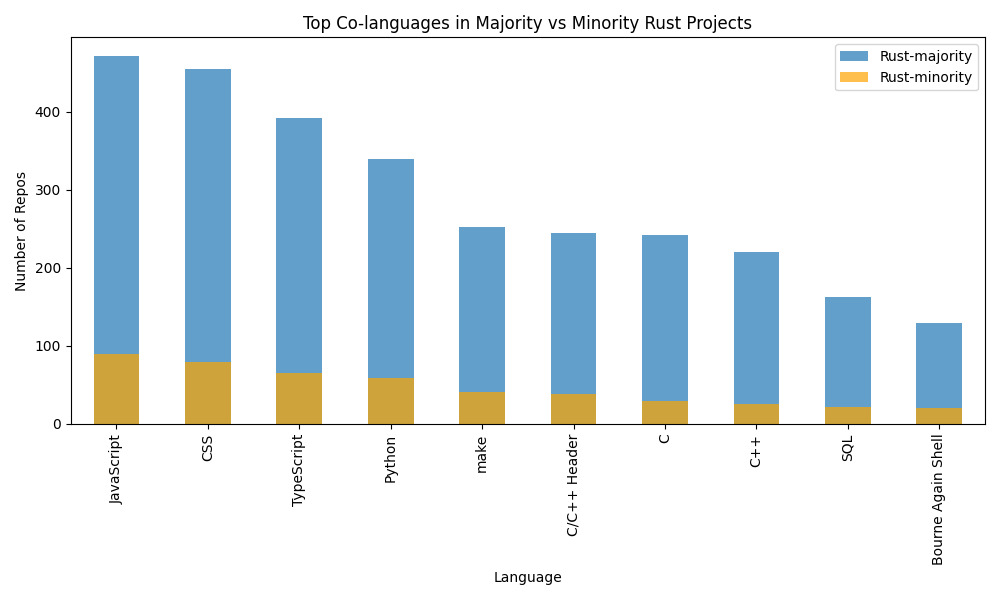
\includegraphics[width=.9\linewidth]{./figures/colanguage_counts_majority_vs_minority.jpg}
\end{center}

\subsection{Commit Frequency}
\begin{tabularx}{\linewidth}{@{}XX@{}}
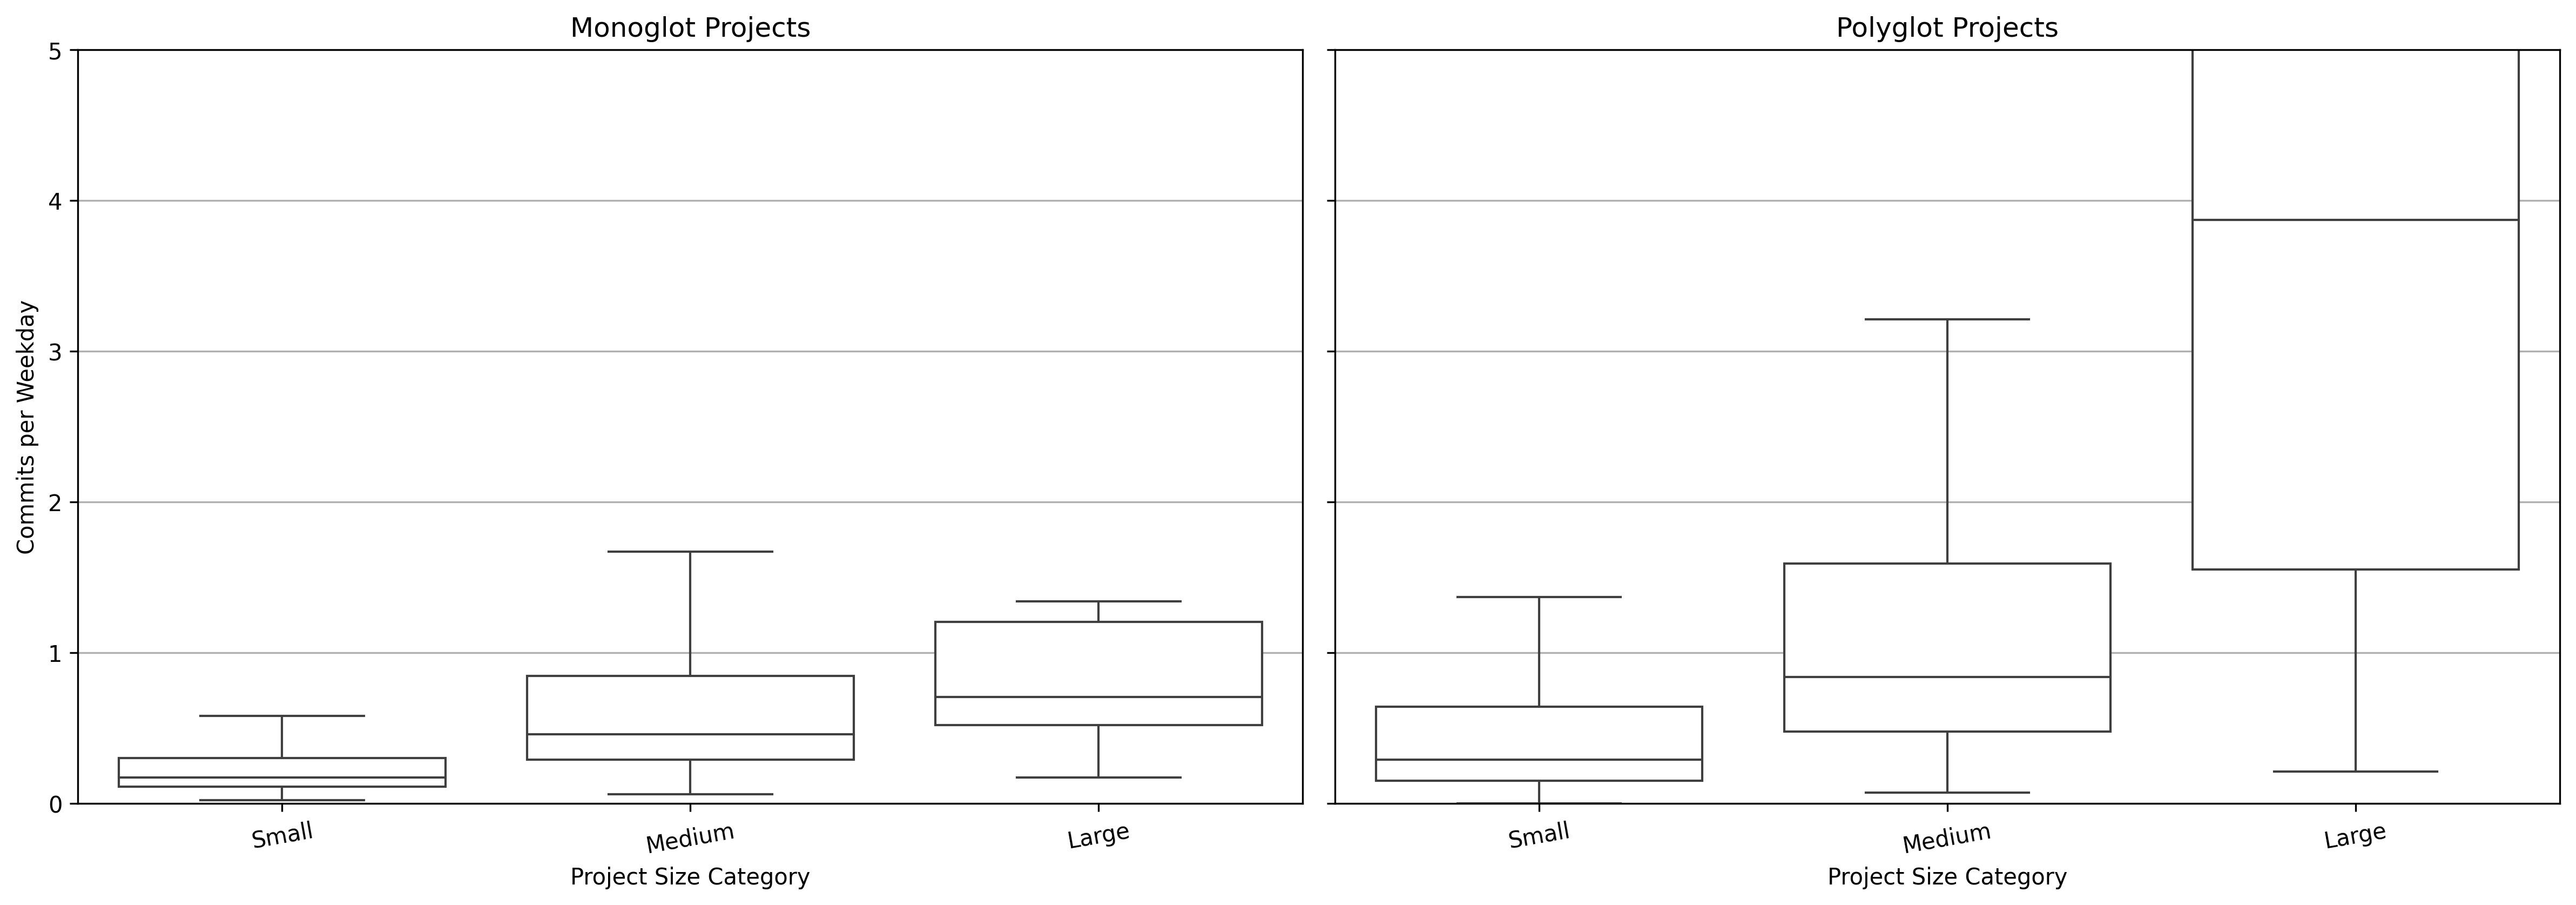
\includegraphics[width=\linewidth]{figures/commit_freq.jpg}
\end{tabularx}
\begin{center}
\begin{tabular}{llrrr}
Cohort & Size & Mean & First Quartile & Third Quartile\\
\hline
Monoglot & Large & 1.61 & 0.52 & 1.20\\
Monoglot & Medium & 0.73 & 0.29 & 0.84\\
Monoglot & Small & 0.33 & 0.11 & 0.30\\
Polyglot & Large & 6.04 & 1.55 & 6.96\\
Polyglot & Medium & 1.41 & 0.48 & 1.59\\
Polyglot & Small & 0.60 & 0.15 & 0.64\\
\end{tabular}
\end{center}
We can see a strong correlation between project size and commit frequency for both monoglot and polyglot Rust projects. In both cohorts, larger projects tend to have a higher mean number of commits per weekday. Polyglot rust projects consistently exhibit a much higher commit frequency than their monoglot counterparts across all size categories. The median commit rate for large polyglot projects is nearly five times that of large monoglot projects (6.96 vs. 1.20). This could point to more diverse and active development teams in these multi-language environments. Polyglot projects often have a broader contributor base with diverse skill sets (e.g., front-end web developers using JavaScript and back-end systems developers using Rust) who are working on different components in parallel. This concurrent development workflow inherently leads to more frequent commits and a greater number of merges into the main branch, a key characteristic of the polyglot Rust ecosystem.

Conversely, the monoglot cohort, particularly the small and medium-sized projects, exhibits much lower commit frequencies. This aligns with the ``CI Theater'' anti-pattern of infrequent commits, which can lead to delayed feedback and larger, more complex merges.  A potential explanation for this low frequency is that these projects are in a maintenance or legacy phase, where major feature development is complete and the codebase is stable, leading to infrequent, targeted commits for bug fixes or minor updates.

\subsection{Broken Build Duration}
\begin{tabularx}{\linewidth}{@{}XX@{}}
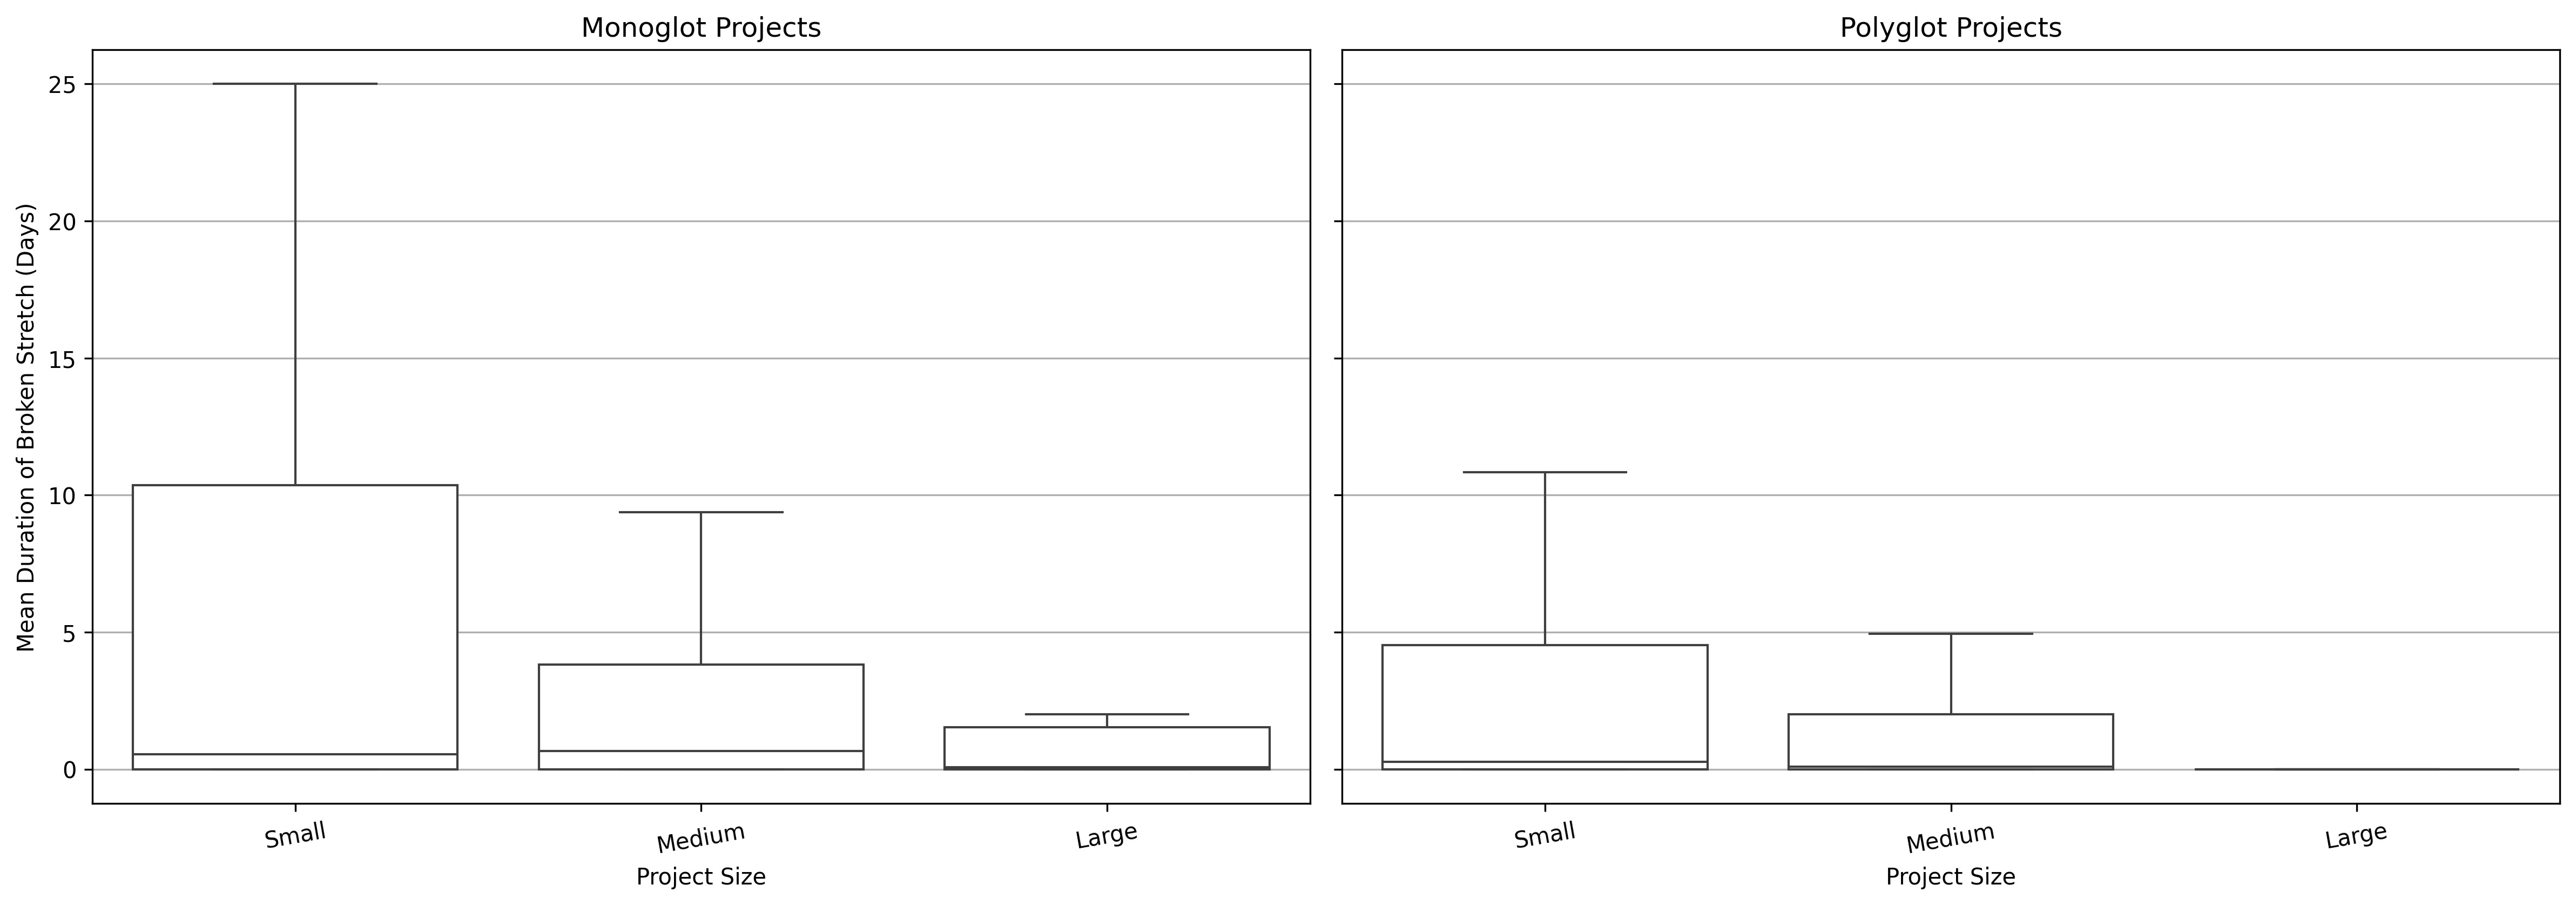
\includegraphics[width=\linewidth]{figures/broken_build_duration.jpg}
\end{tabularx}
\begin{center}
\begin{tabular}{llrrr}
Cohort & Size & Mean (days) & Count & Std. Dev.\\
\hline
Monoglot & Small & 27.39 & 328 & 76.58\\
Monoglot & Medium & 10.30 & 164 & 40.29\\
Monoglot & Large & 5.27 & 6 & 11.90\\
Polyglot & Small & 22.97 & 530 & 72.43\\
Polyglot & Medium & 14.77 & 788 & 60.14\\
Polyglot & Large & 1.92 & 194 & 11.65\\
\end{tabular}
\end{center}
Broken build analysis across Rust projects reveals few contrasts between monoglot and polyglot cohorts, with small projects in both categories exhibiting highly skewed distributions. In monoglot small projects, the mean duration of a broken build stretch is 27.39 days, yet the median is only 0.55 days, signaling that while most projects recover quickly, a minority suffer extended downtime. These long tails visible in both mean and standard deviation suggest that CI neglect or lack of contributor activity leaves smaller monoglot repositories especially vulnerable to “CI theater” behaviors, such as unrepair-ed main branches and stagnation. Medium and large monoglot projects gradually reduce both mean and median broken build durations, but occasional outliers persist which keeping averages elevated. The results reinforce prior findings that healthy CI practice depends on both team engagement and automation, and imply that focused investment in CI pipeline reliability especially for small projects could reduce extended failures in the Rust ecosystem.

\subsection{Build Duration}
\begin{tabularx}{\linewidth}{@{}XX@{}}
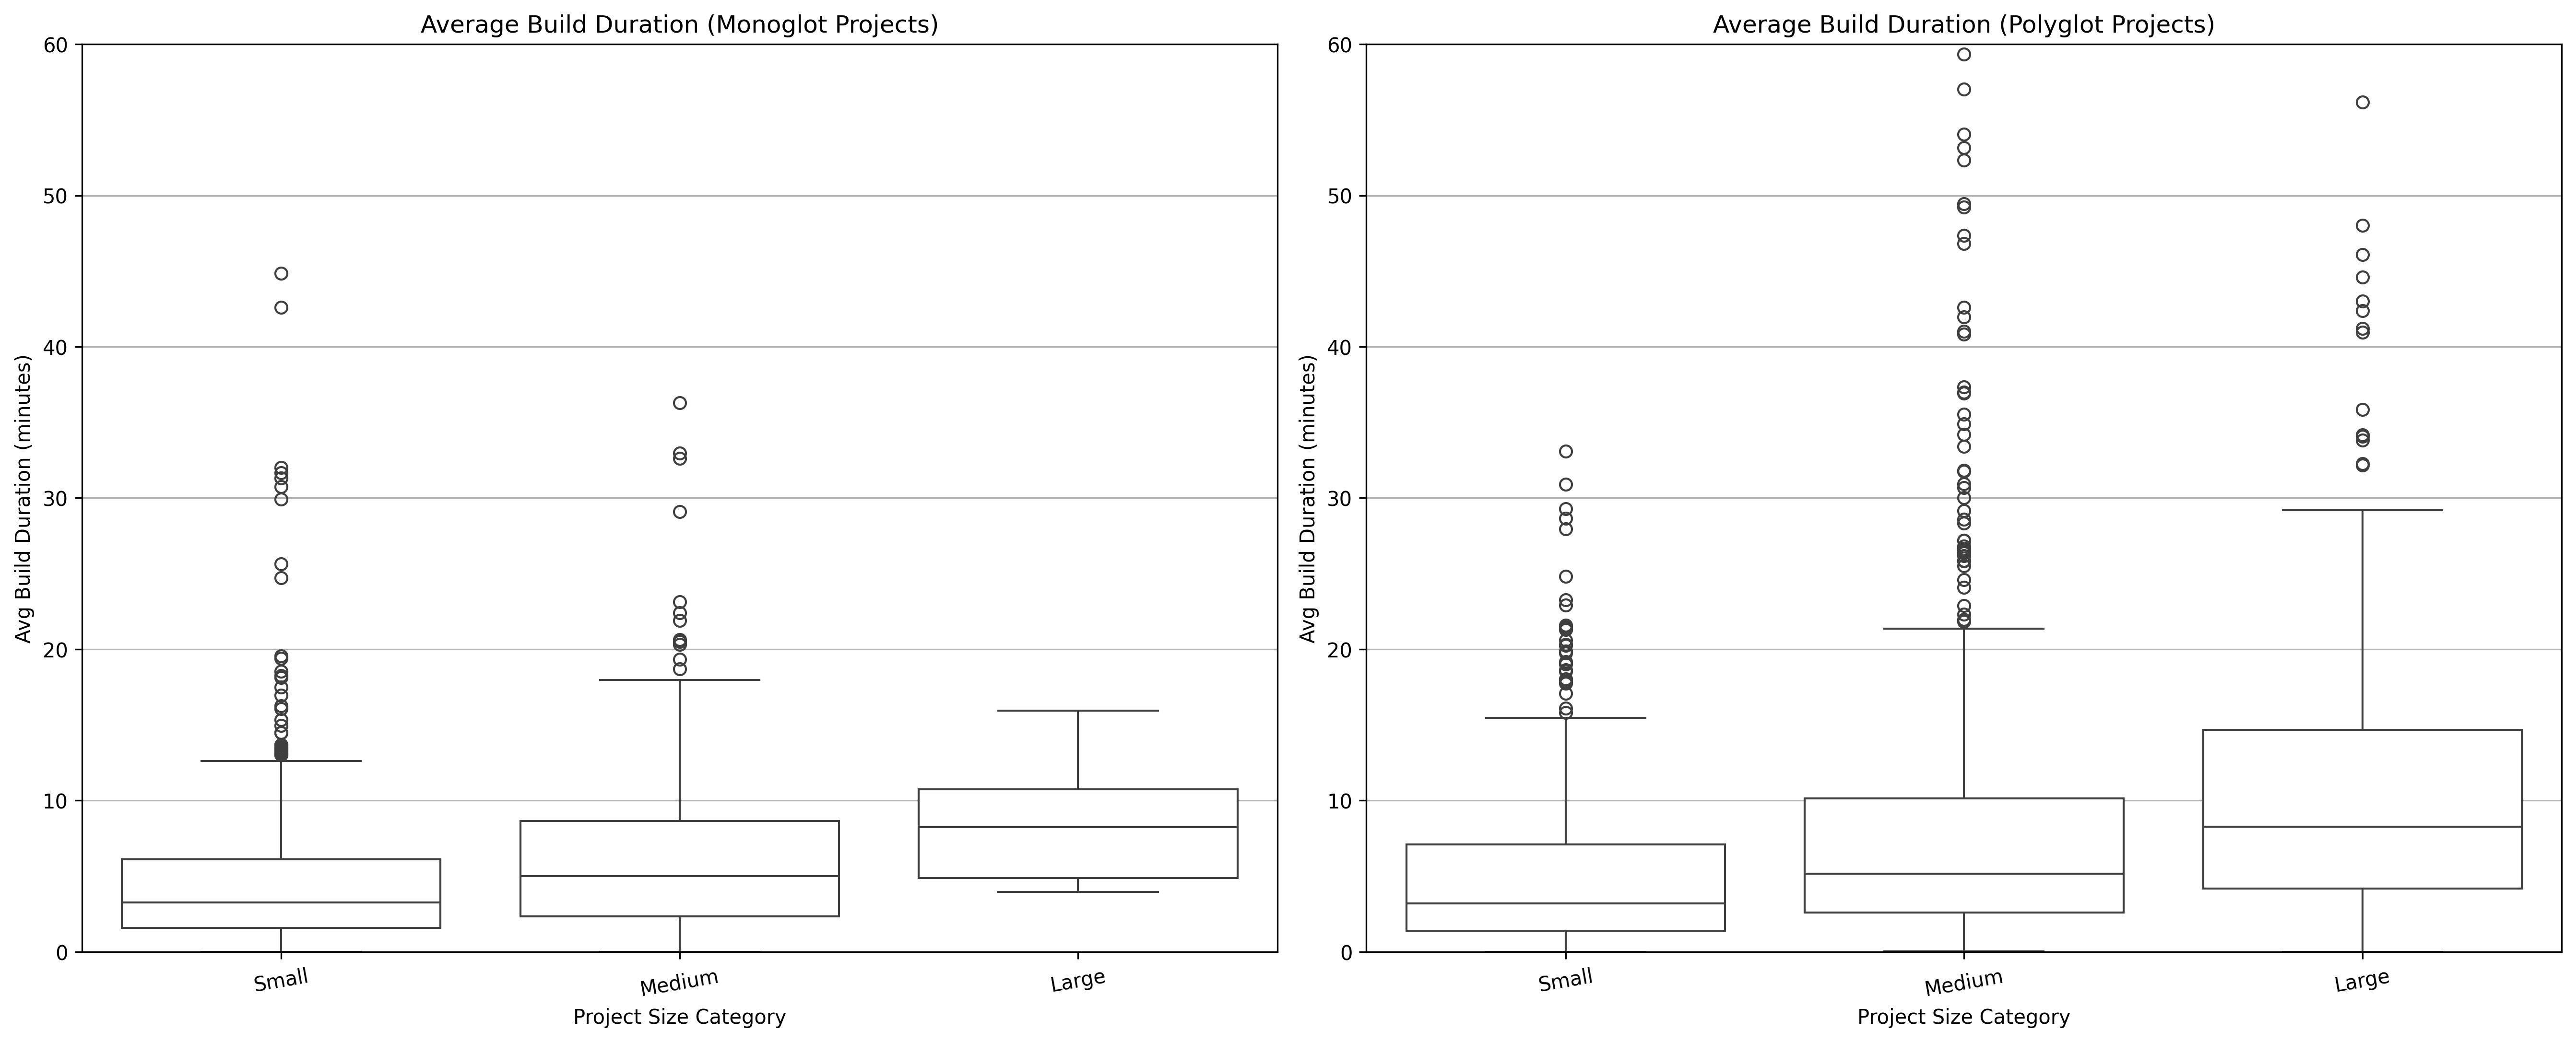
\includegraphics[width=\linewidth]{figures/build_duration.jpg}
\end{tabularx}
\begin{center}
\begin{tabular}{llrrrr}
Cohort & Category & Mean & Median & 1st Quartile & 3rd Quartile\\
\hline
Monoglot & Small & 5.58 & 3.270 & 1.58 & 6.12\\
Monoglot & Medium & 7.28 & 5.000 & 2.35 & 8.64\\
Monoglot & Large & 8.62 & 8.245 & 4.89 & 10.73\\
Polyglot & Small & 5.44 & 3.195 & 1.40 & 7.09\\
Polyglot & Medium & 8.32 & 5.160 & 2.59 & 10.15\\
Polyglot & Large & 11.23 & 8.260 & 4.18 & 14.69\\
\end{tabular}
\end{center}

For small projects, both cohorts report similar mean build times of around 5.5 minutes. This is slightly longer than the average of 4 minutes and 18 seconds observed in the Continuous Integration Theater study of Java and Ruby projects \autocite{felidre2019ci_theater}. The gap widens with size, as medium and large polyglot projects face notably longer average build durations, with a mean of 11.2 minutes for large projects. This tendency for large, complex projects to have longer build times mirrors the findings from the CI Theater paper, which noted that over half of large Java projects also breached the 10-minute threshold.

Despite these higher averages in Rust projects, the median build times remain remarkably similar across both cohorts, which underscores that the difference is driven by outliers rather than a slower typical build. Box plot visualizations confirm this trend, showing that most builds cluster under 10 minutes, similar to the earlier study where only 16% of projects had long-running builds. However, a minority of large polyglot Rust projects experience runs extending over 15 minutes.

These sustained build durations likely reflect the CI complexity and multi-language orchestration in polyglot projects, where additional linting, cross-language compilation, and integration tasks may stretch runtime. In contrast, monoglot Rust projects maintain steadier scaling with fewer extreme outliers. These results suggest that while build times for small projects are comparable regardless of language mix, the longer durations for large and medium polyglot projects may be a key target for CI optimization—potentially through caching, parallelization, and focused workflow engineering.

\subsection{Test Coverage Adoption}
\begin{tabularx}{\linewidth}{@{}XX@{}}
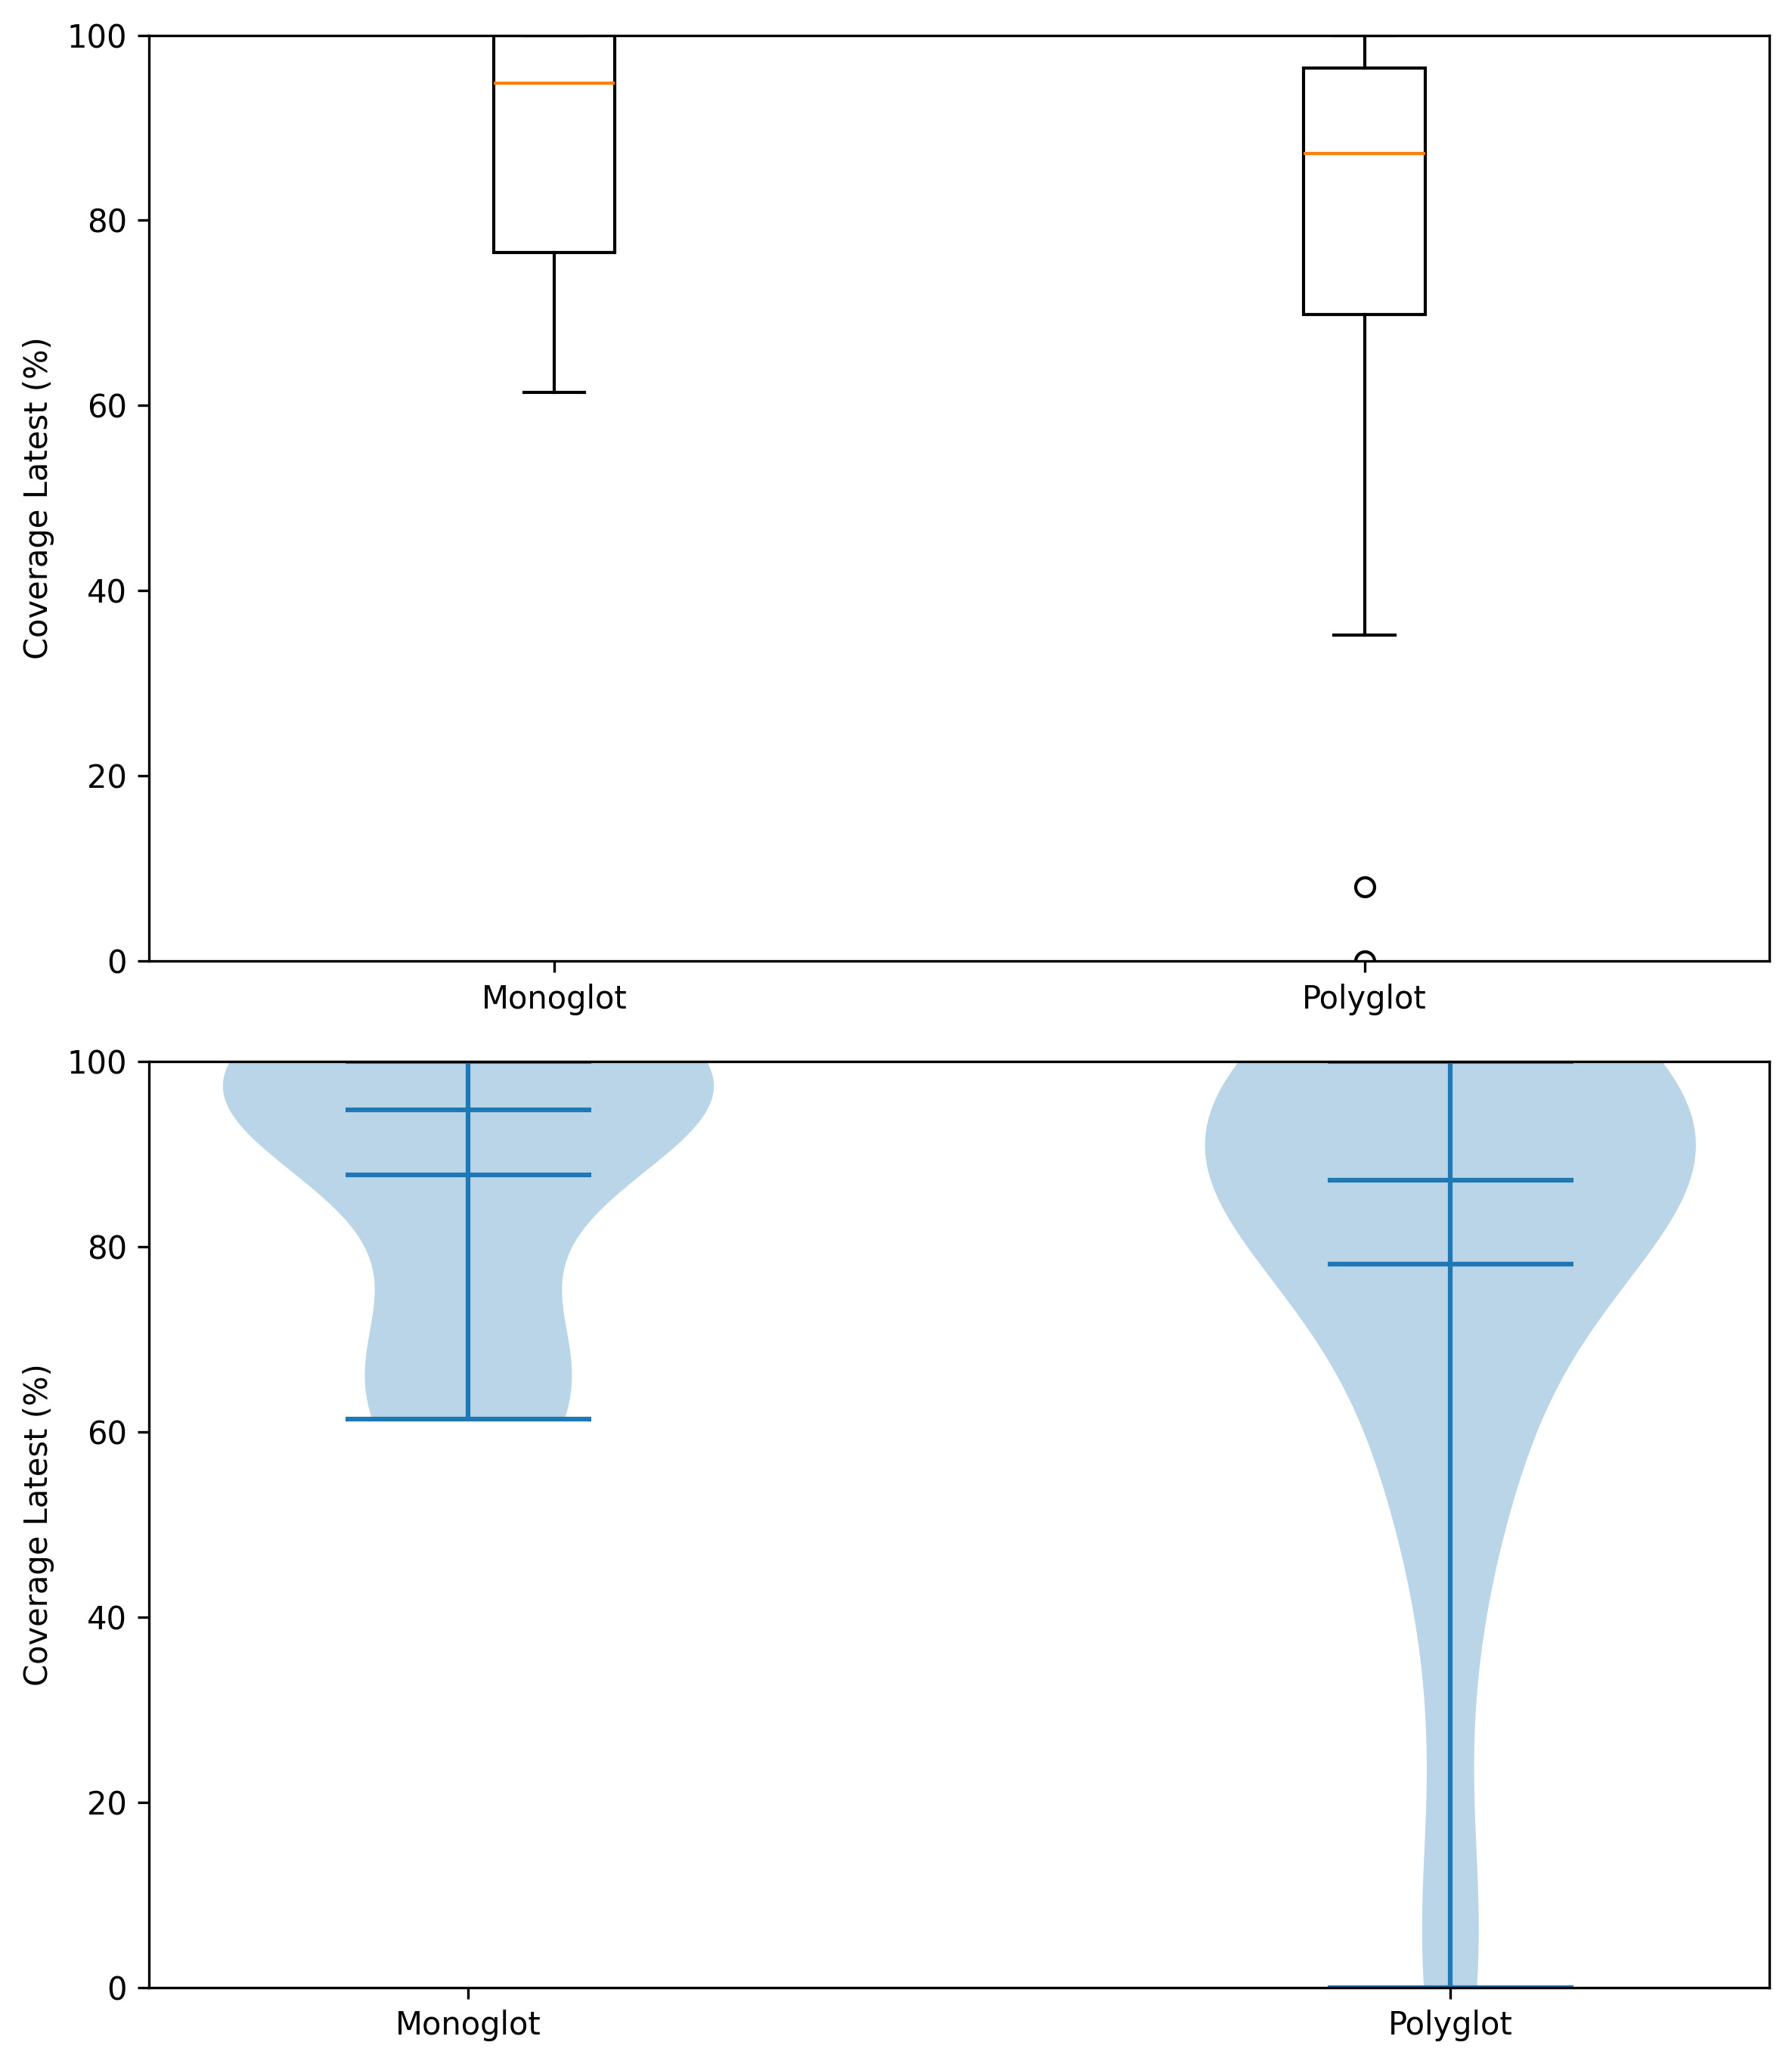
\includegraphics[width=\linewidth]{figures/test_coverage.jpg} &
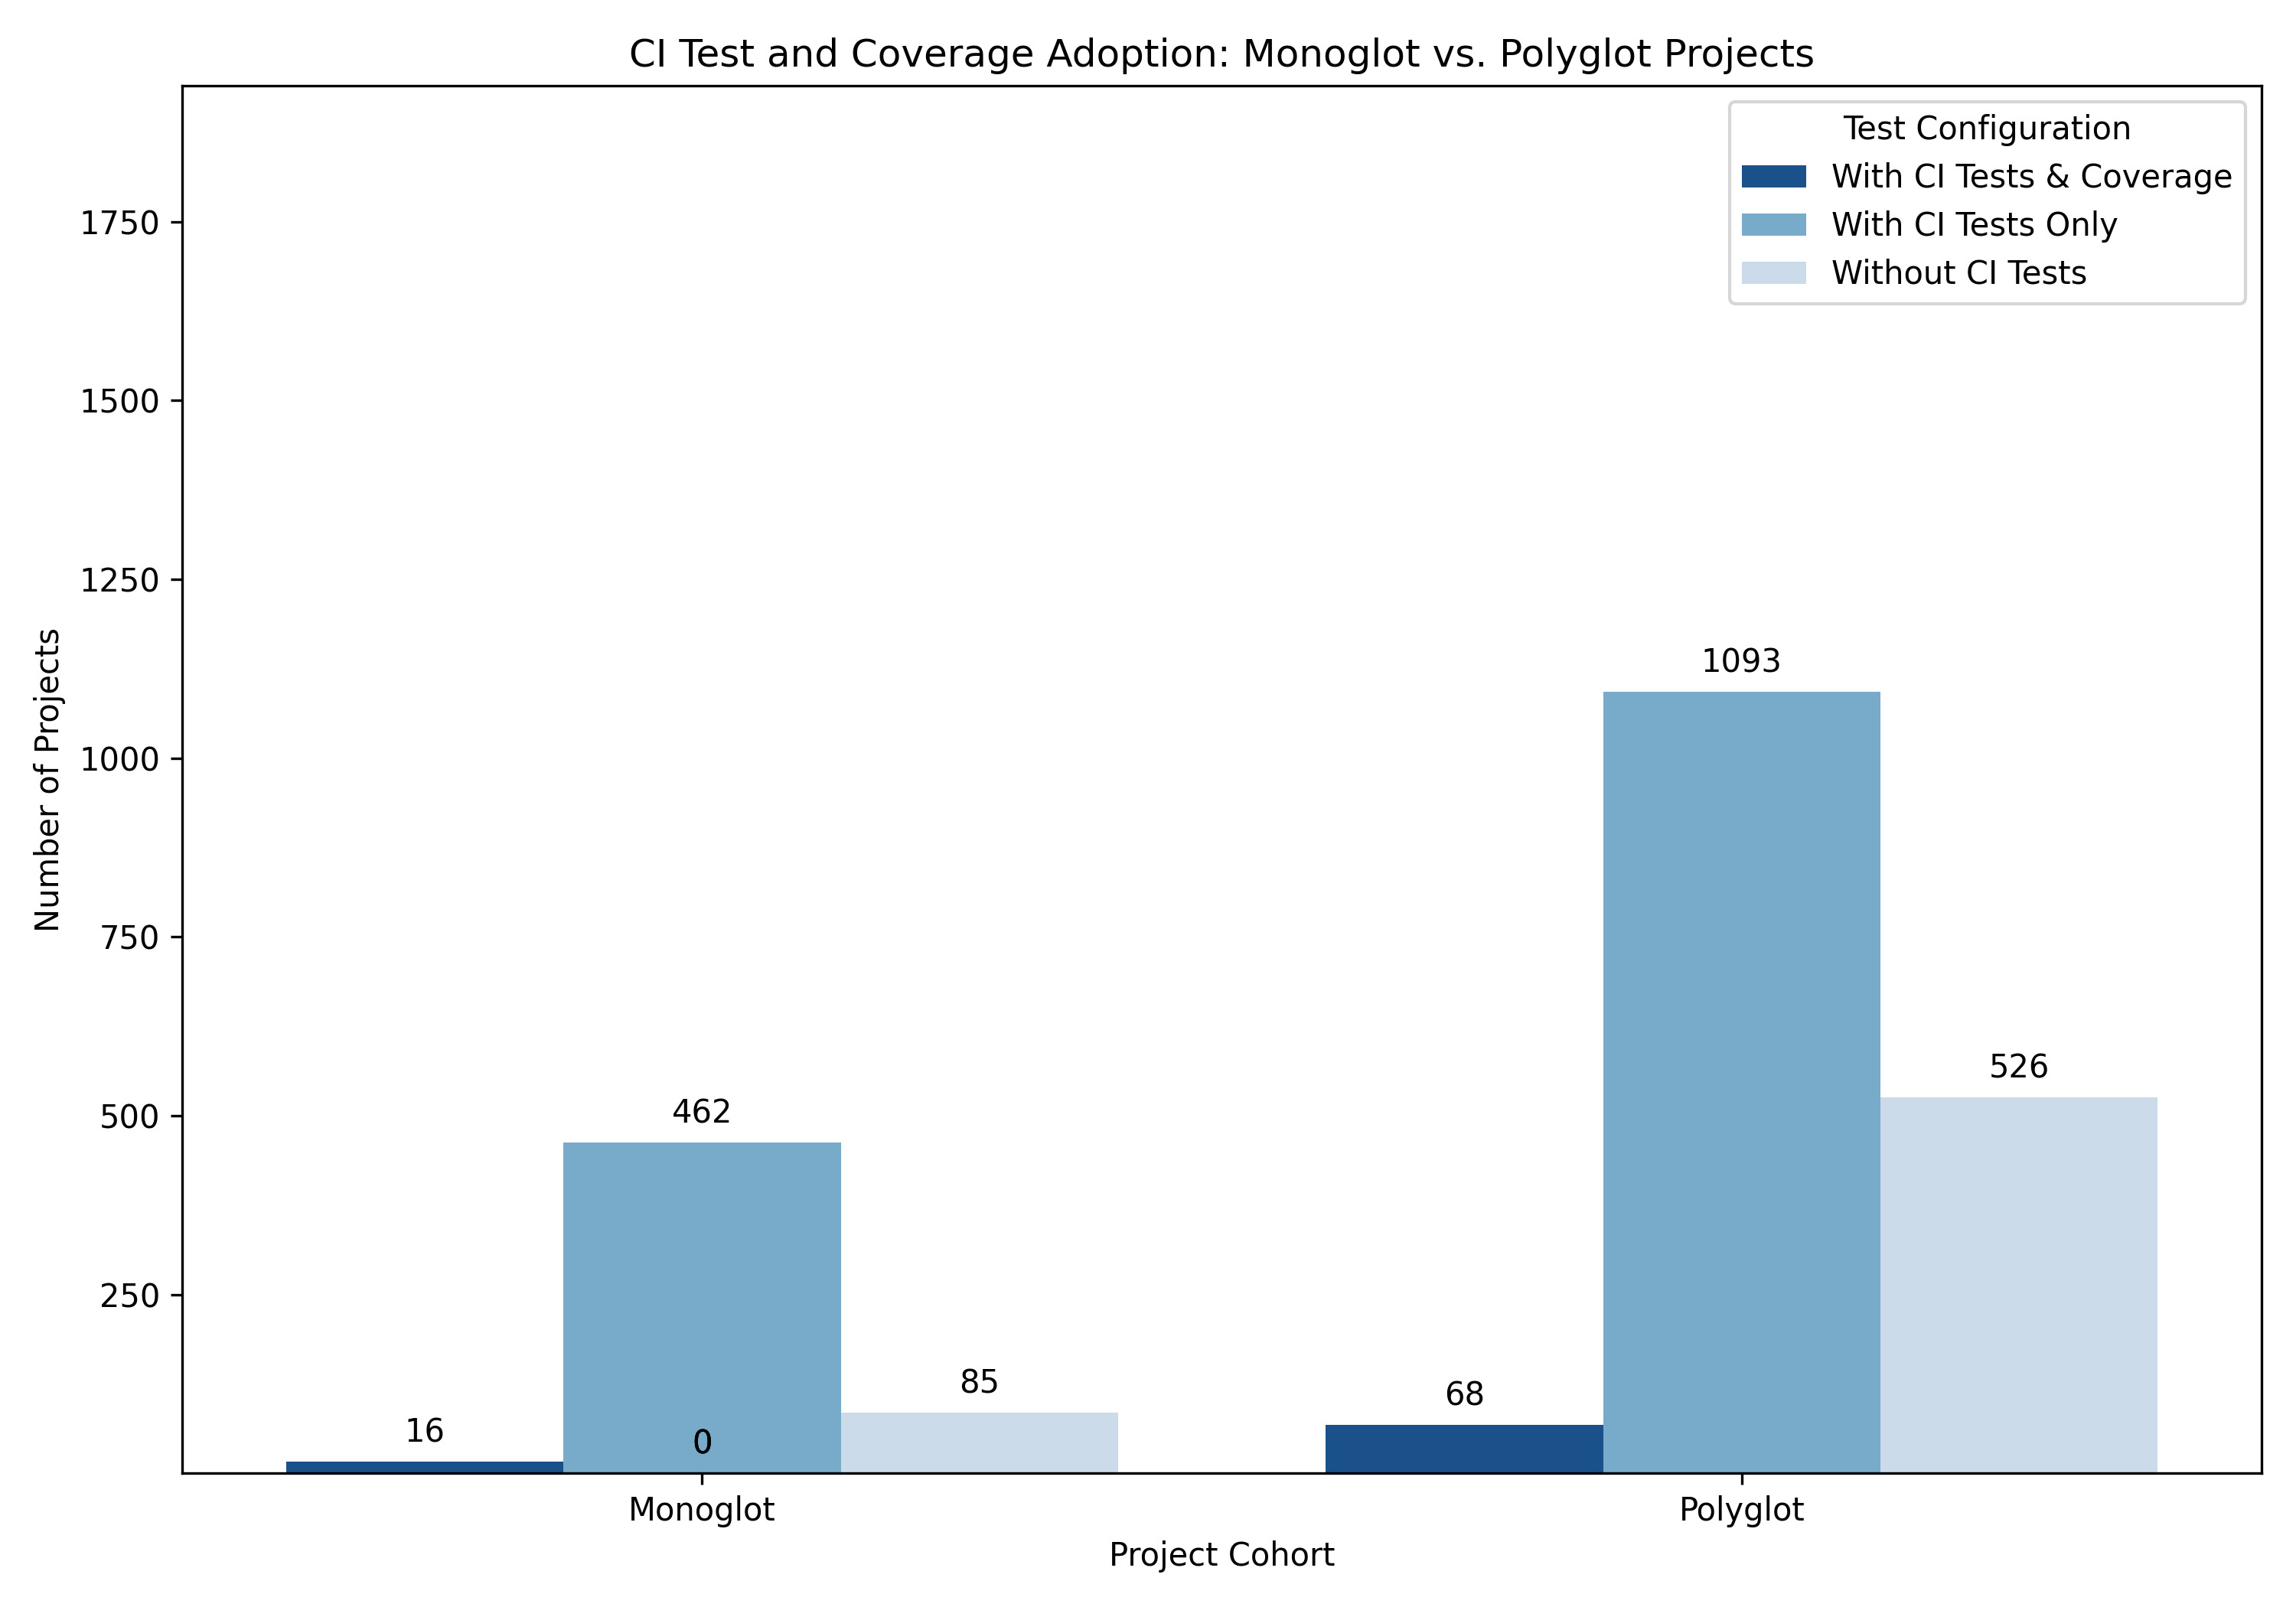
\includegraphics[width=\linewidth]{figures/ci_test_adoption.jpg} &
\end{tabularx}
\begin{center}
\begin{tabular}{lrrr}
Cohort & Mean & 1st Quartile & 3rd Quartile\\
\hline
Monoglot & 87.79 & 76.50 & 100.00\\
Polyglot & 78.12 & 69.80 & 96.44\\
\end{tabular}
\end{center}
Test coverage in Rust projects shows clear differences between monoglot and polyglot repositories. Monoglot projects tend to have higher and more consistent coverage, with a mean of 87.8\% and a third quartile of 100\%, indicating strong testing practices. Polyglot projects, while capable of high coverage (third quartile 96.4\%), show greater variability and a lower mean (78.1\%), likely due to the complexity of multi-language CI setups. CI test adoption is widespread: 462 monoglot and 1093 polyglot projects have CI tests. However, meaningful coverage is rare overall. Only 3.05\% of monoglot and 5.05\% of polyglot projects have coverage configured and report non-zero samples. That leaves 540 monoglot and 1334 polyglot projects without actionable coverage data. While many Rust projects adopt CI testing, most do not track coverage effectively highlighting a gap in tooling, enforcement, or prioritization.

\subsection{CI Adoption Velocity}
\begin{tabularx}{\linewidth}{@{}XX@{}}
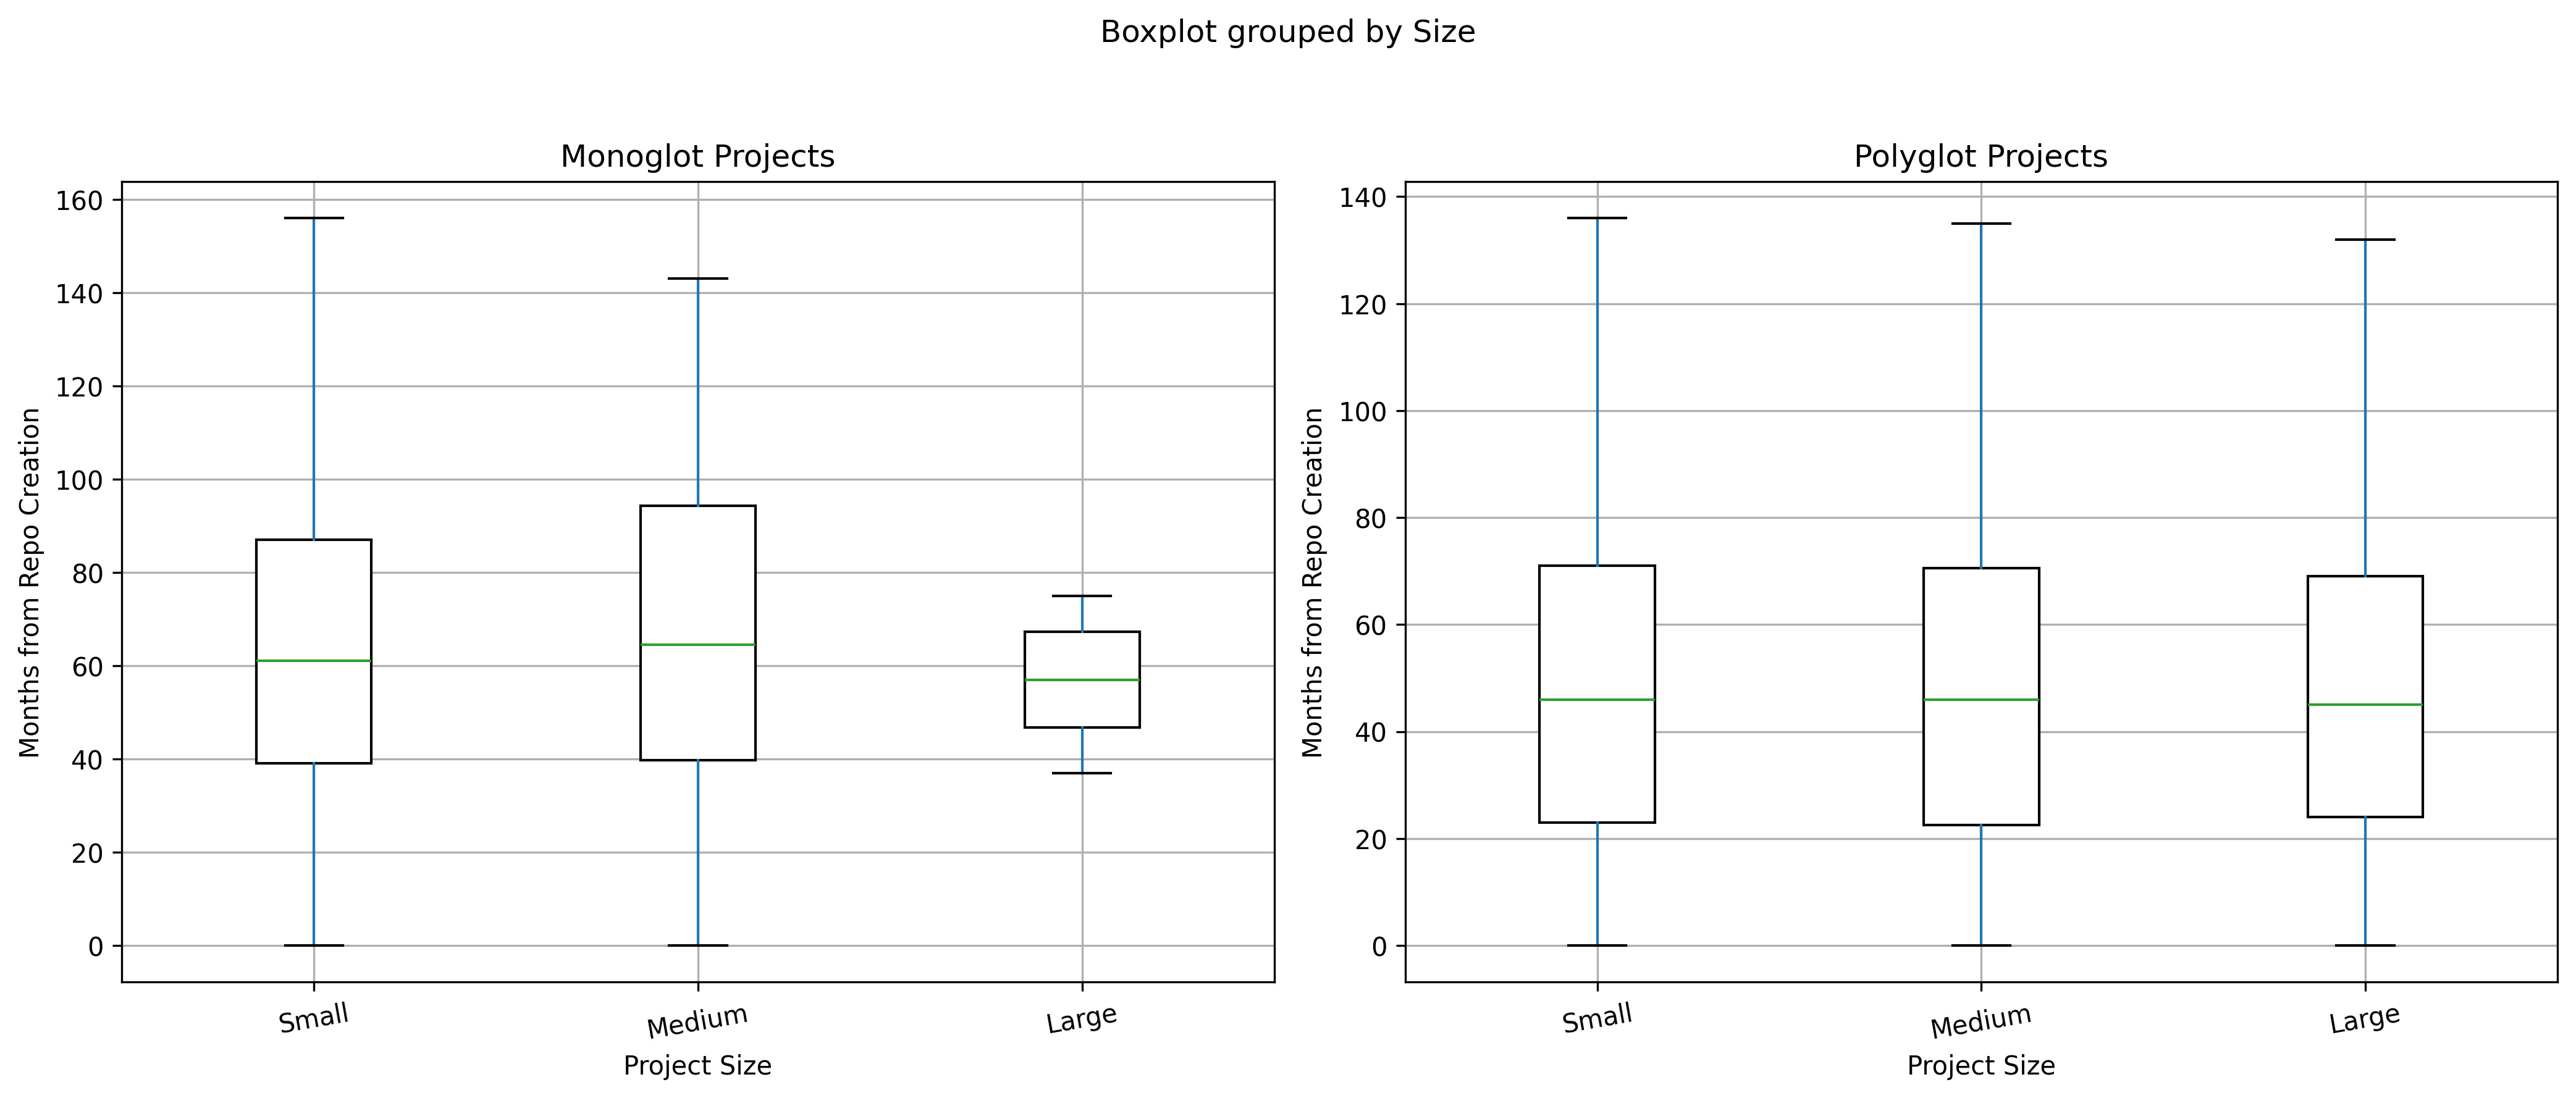
\includegraphics[width=\linewidth]{figures/time_to_ci.jpg}
\end{tabularx}
\begin{center}
\begin{tabular}{llrrr}
Cohort & Size & Mean & Q1 & Q3\\
\hline
Monoglot & Small & 63.64 & 39.00 & 87.00\\
Monoglot & Medium & 66.01 & 39.75 & 94.25\\
Monoglot & Large & 56.67 & 46.75 & 67.25\\
Polyglot & Small & 49.05 & 23.00 & 71.00\\
Polyglot & Medium & 49.82 & 22.50 & 70.50\\
Polyglot & Large & 47.63 & 24.00 & 69.00\\
\end{tabular}
\end{center}
Rust projects exhibit notably slow adoption of continuous integration (CI) compared to industry standards in other open-source ecosystems. For monoglot (pure Rust) projects, the average lag before first CI setup is especially long—over 5 years for most size categories, and more than 7 years for many medium-sized projects. This means many pure Rust repositories delay implementing automated builds and tests for several years, suggesting that CI is often de-prioritized within much of the Rust ecosystem.

By contrast, a study by \autocite{Hilton2016} found that in general open-source projects, the median time to adopt CI is about one year after project inception. Polyglot projects in the Rust ecosystem adopt CI somewhat faster and with less variation (around 4 years on average), but still lag behind industry best practices where CI is ope-rationalized within months. This persistence of delayed adoption underlines the need for Rust projects to prioritize earlier CI setup to improve project health and reliability.

\begin{figure}[htbp]
  \centering
  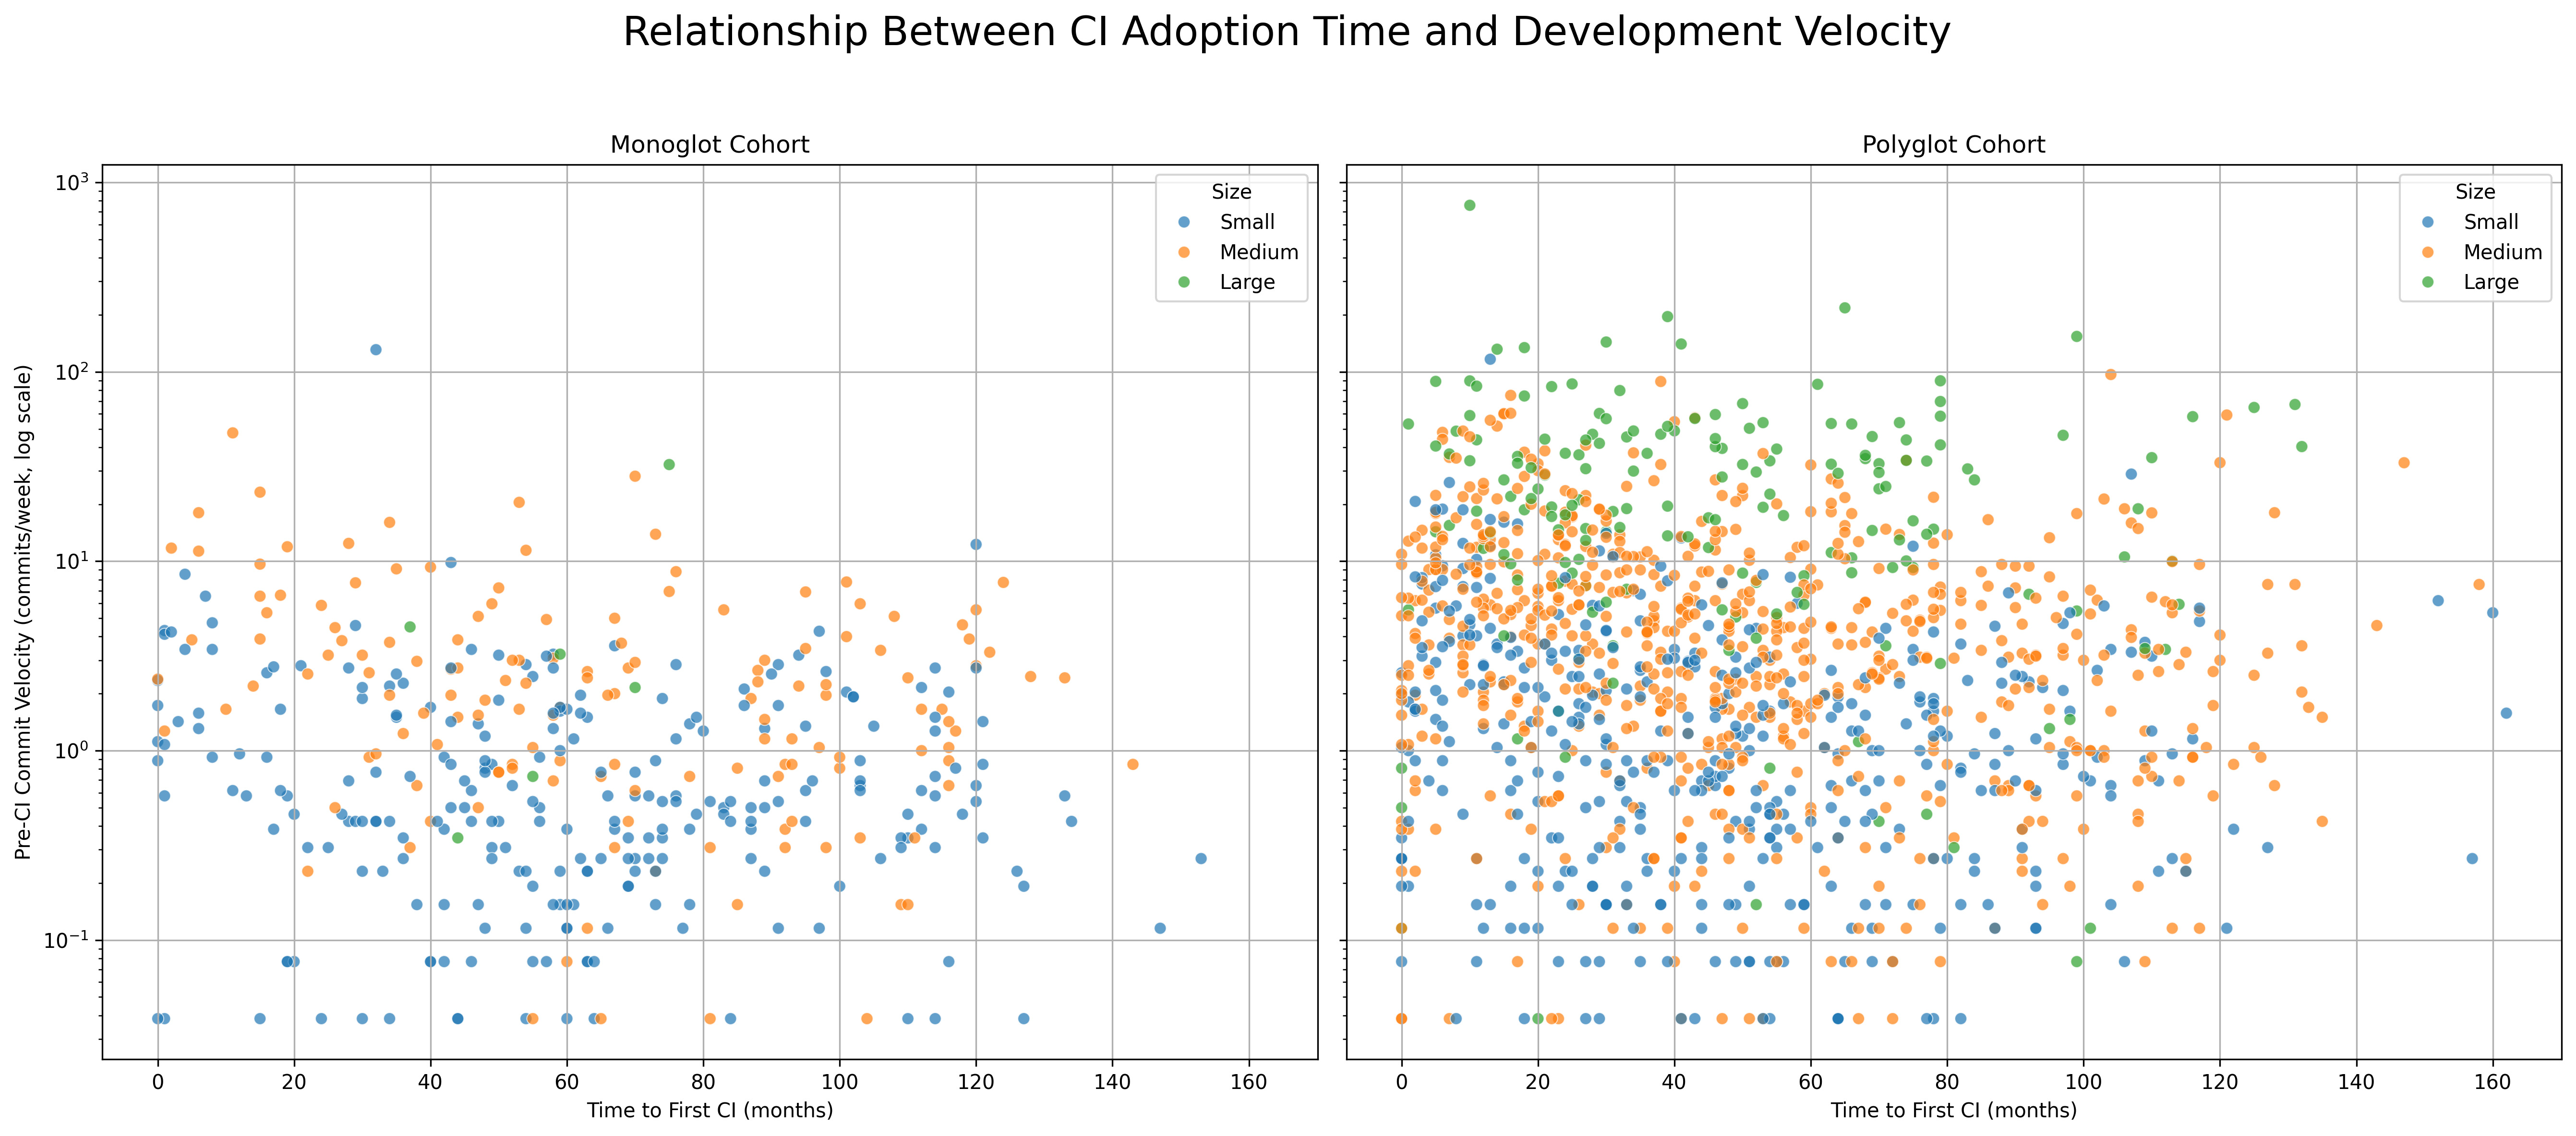
\includegraphics[width=\linewidth]{figures/ci_correlation_plot.jpg}
  \caption{CI correlation plot for Rust project cohorts.}
  \label{fig:ci_correlation_plot}
\end{figure}

\begin{table}[htbp]
\centering
\caption{Consolidated Descriptive Statistics for Project Cohorts}
\label{tab:cohort_stats_consolidated}
\begin{tabular}{llrr}
\toprule
\textbf{Cohort} & \textbf{Statistic} & \textbf{Velocity} & \textbf{Time to First CI (months)} \\
\midrule
Monoglot & Mean          & 2.02     & 64.33    \\
Monoglot & Std. Dev.     & 6.95     & 34.25    \\
Monoglot & 25\%          & 0.12     & 39.50    \\
Monoglot & 50\% (Median) & 0.58     & 62.00    \\
Monoglot & 75\%          & 1.96     & 90.50    \\
Monoglot & Max           & 130.92   & 156.00   \\
\midrule
Polyglot & Mean          & 8.61     & 49.23    \\
Polyglot & Std. Dev.     & 26.06    & 33.31    \\
Polyglot & 25\%          & 0.38     & 23.00    \\
Polyglot & 50\% (Median) & 2.27     & 46.00    \\
Polyglot & 75\%          & 7.54     & 70.00    \\
Polyglot & Max           & 757.38   & 162.00   \\
\bottomrule
\end{tabular}
\end{table}

The consolidated statistics reveal differences in development velocity preceding CI adoption between monoglot and polyglot Rust projects. Monoglot projects demonstrate lower velocity metrics, with a mean of 2.02 commits per weekday and a median of 0.58 commits per weekday during the period leading to CI implementation. The distribution shows that 75% of monoglot projects maintain commit rates below 1.96 commits per weekday, while 25% operate at extremely low frequencies of 0.12 commits per weekday or less. The maximum recorded velocity of 130.92 commits per weekday represents an outlier, indicating that while most monoglot projects exhibit minimal development activity before CI adoption, a small subset maintains exceptionally high commit frequencies.

Polyglot projects exhibit higher development velocity preceding CI adoption, with a mean of 8.61 commits per weekday and a median of 2.27 commits per weekday. The first quartile maintains 0.38 commits per weekday, while the third quartile reaches 7.54 commits per weekday, demonstrating consistently higher activity levels across the distribution. The maximum velocity of 757.38 commits per weekday, while extreme, reflects the capacity for high-frequency development in polyglot. These velocity differences correlate directly with CI adoption timelines, where monoglot projects delay CI implementation for a median of 62 months compared to 46 months for polyglot projects. The data demonstrates that projects with higher pre-CI development velocity tend to adopt CI earlier, suggesting that active development patterns drive the need of CI necessity.

\subsection{Defect Rates Before and After CI Adoption}
\begin{tabularx}{\linewidth}{@{}XX@{}}
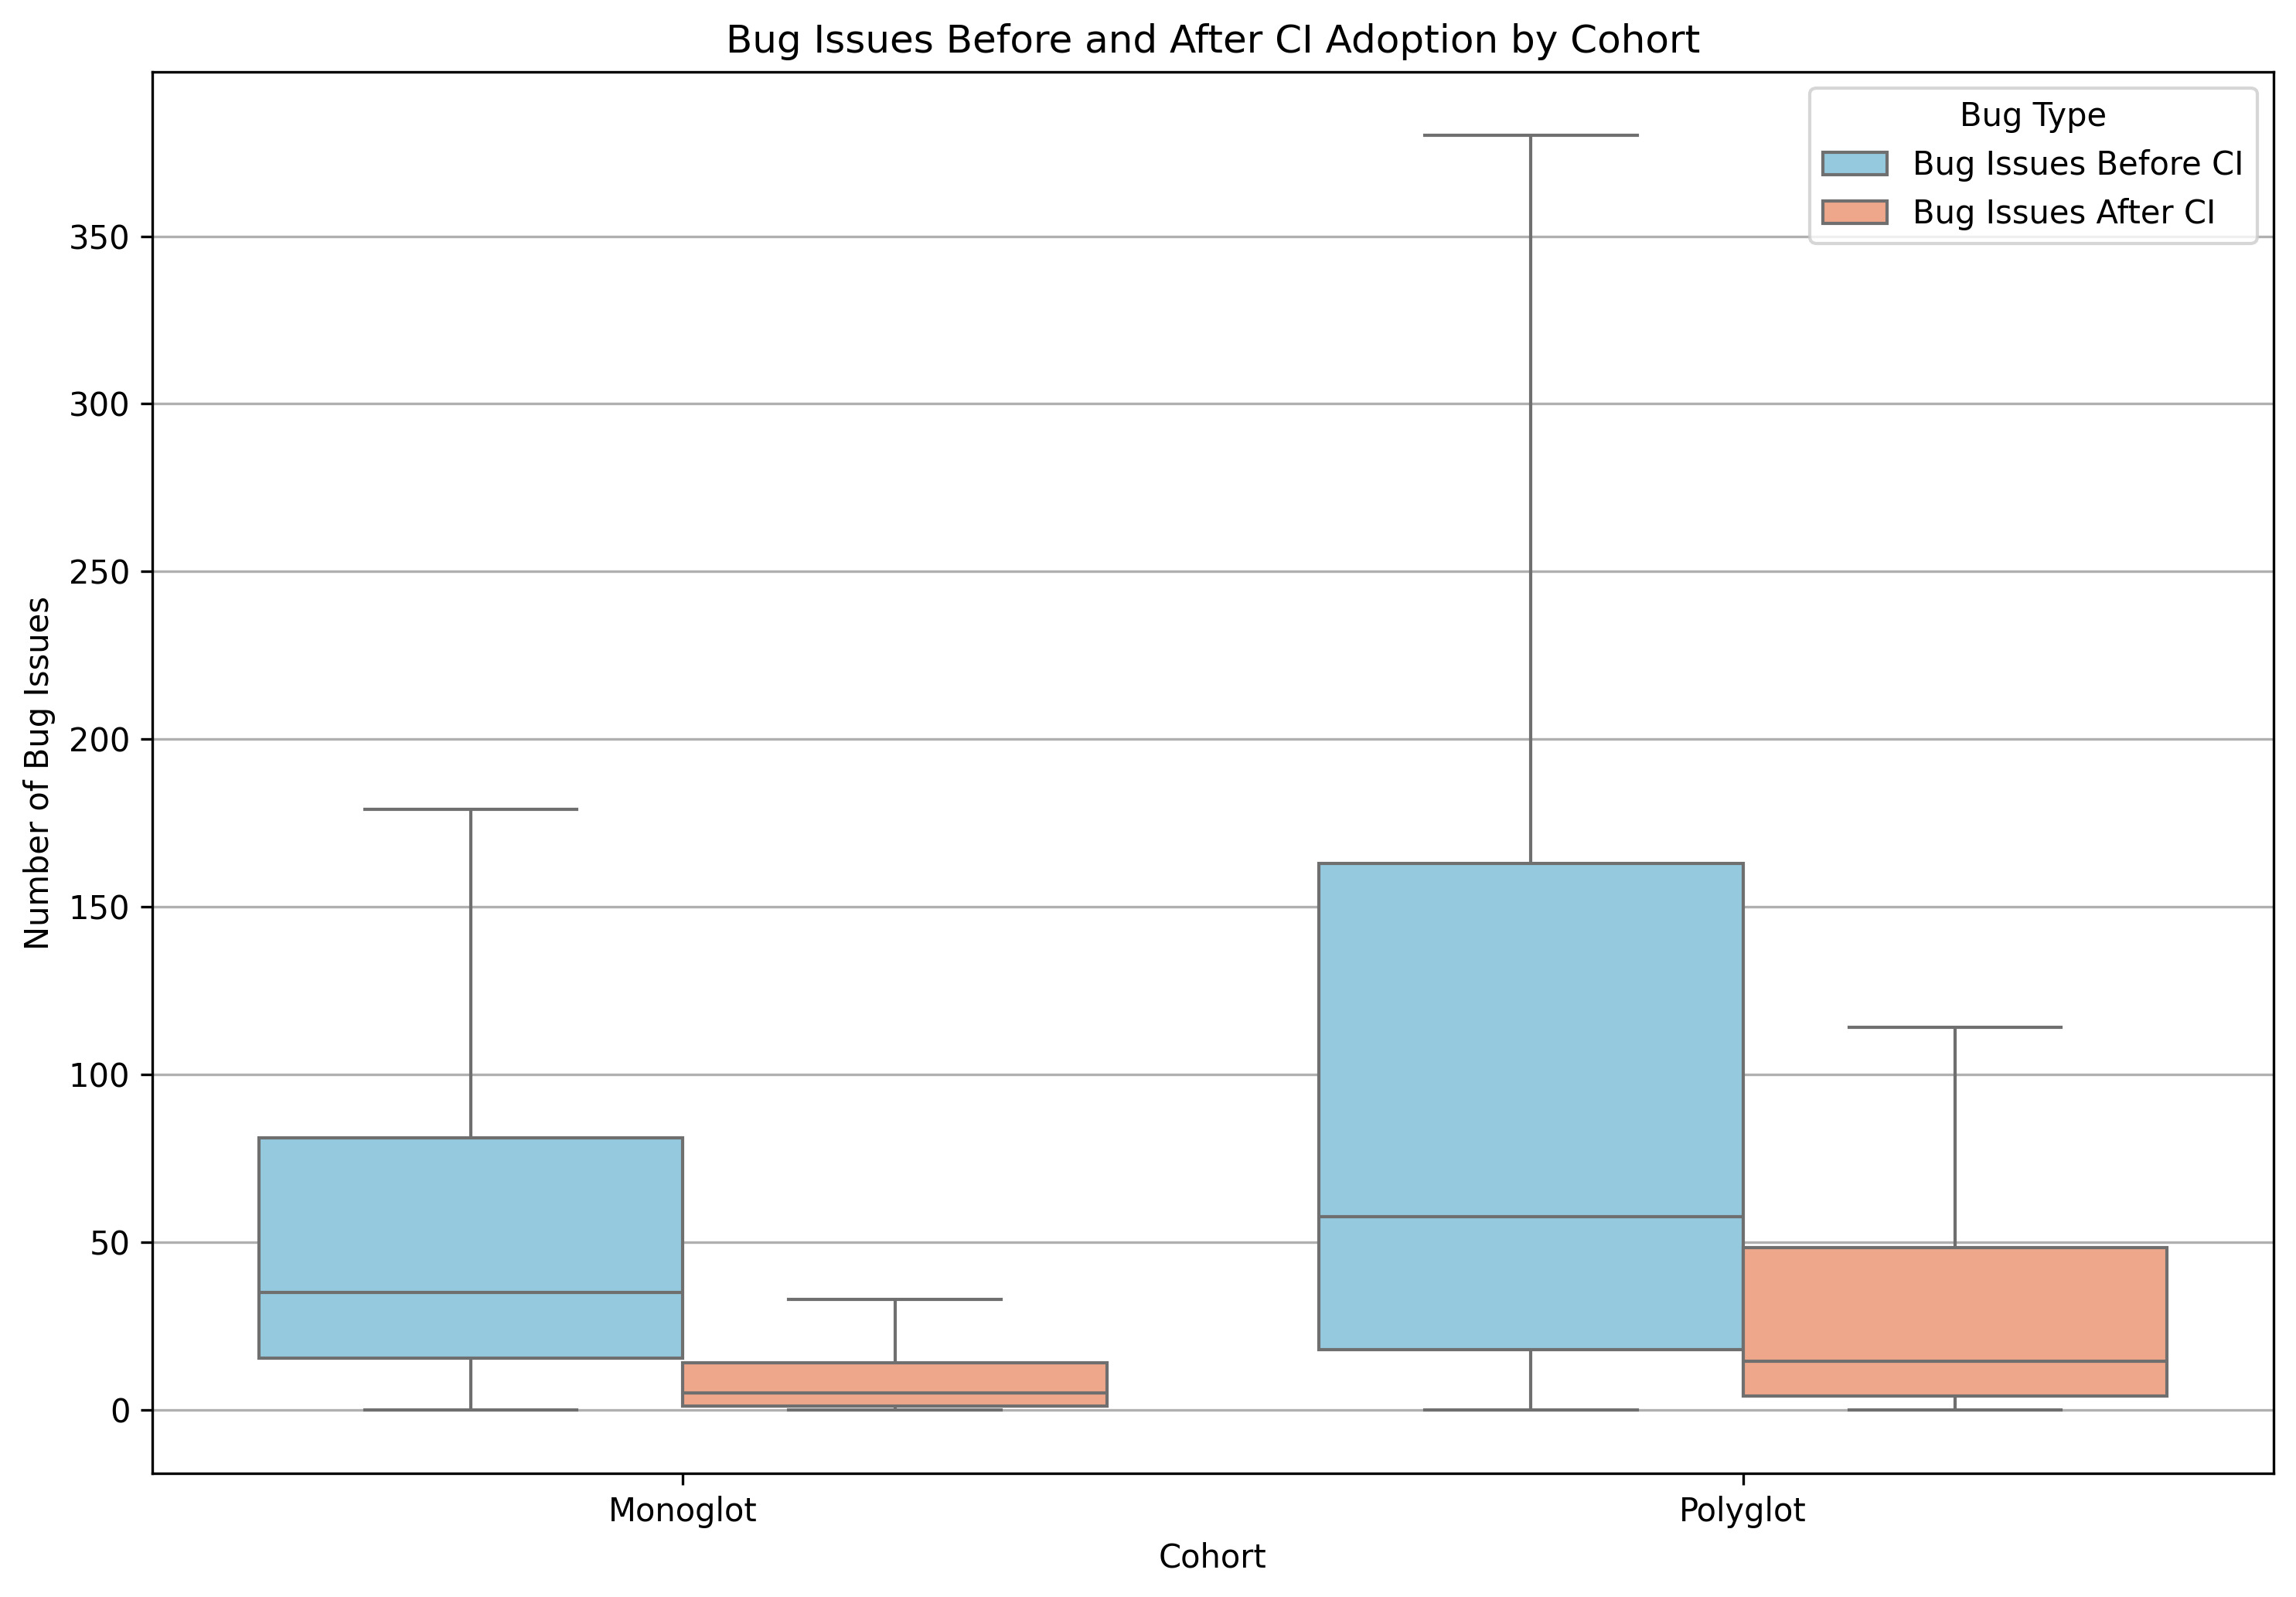
\includegraphics[width=\linewidth]{figures/bugs_before_after_ci_by_cohort.jpg}
\end{tabularx}
\begin{center}
\begin{tabular}{llrrr}
Cohort & Bug Type & Mean & Q1 & Q3\\
\hline
Monoglot & Bug Issues Before CI & 68.21 & 15.5 & 81.00\\
Monoglot & Bug Issues After CI & 12.23 & 1.0 & 14.00\\
Polyglot & Bug Issues Before CI & 170.60 & 18.0 & 163.00\\
Polyglot & Bug Issues After CI & 72.99 & 4.0 & 48.25\\
\end{tabular}
\end{center}
The statistics for bug issues before and after CI adoption show a substantial reduction in reported bugs for both monoglot and polyglot Rust projects following the introduction of continuous integration. For monoglot projects, the average number of bug issues drops from 68.2 before CI to just 12.2 after CI, with the first quartile declining from 15.5 to 1.0 and the third quartile dropping from 81.0 to 14.0. This pattern indicates that most pure Rust projects experience fewer bug reports after integrating CI, and the effect is consistent across both the lower and upper ends of the distribution.

Polyglot projects, which generally report more bugs due to their larger size or complexity, also see a clear decrease. The mean bug issues fall from 170.6 prior to CI to 73.0 following CI adoption. The reduction in the first quartile (18.0 to 4.0) and the third quartile (163.0 to 48.3) highlights that this improvement holds across a wide range of project profiles, though the typical polyglot project still has more bug issues than its monoglot counterpart in both periods. These trends strongly suggest that adopting CI workflows correlates with improved defect management and possibly better software quality in open-source Rust projects.

\section{Discussion}

\subsection{Limitations}
This study has several limitations that should be considered when interpreting findings.

\textbf{Internal Validity}: The study is observational and identifies correlations, not causation. For instance, while we observed a significant reduction in bug-like issues after CI adoption, we cannot definitively conclude that CI was the sole cause. Other factors, such as increased team size, project maturity, or improved development processes, may have also contributed to this outcome.

\textbf{External Validity}: The generalization of results may be limited. The dataset was curated from publicly accessible, open-source projects on GitHub with at least 500 stars. Therefore, the findings may not be representative of private, commercial, or smaller, less popular open-source Rust projects that may have different resources and development practices. Furthermore, as with any repository mining study, the data represents a snapshot in time, the rapidly evolving nature of CI/CD tools and practices means our findings might not fully capture the most current trends in the ecosystem, a limitation common in studies using historical data.

\textbf{Defect Proxy}: The use of issue labels like "bug" or "defect" serves as a proxy for actual software defects. The accuracy of this metric is dependent on the diligence and consistency of the labeling practices within projects.

\textbf{Test Coverage Data}: The analysis of test coverage was based on a very small fraction of projects that reported actionable data (3.05% of monoglot and 5.05% of polyglot projects). This introduces a potential selection bias, as projects that actively report coverage may be more mature or disciplined in their testing practices. This need to rely on proprietary, third-party services for data means we must trust the accuracy of their output, a limitation also noted in previous work.

\textbf{Data Source Reliance}: The study depends on data from the GitHub API and CI logs. The accuracy of metrics like build duration and success is contingent on the reliability of these external systems and the correctness of each project's CI configuration. The potential for missing or incomplete data records from these sources could also affect some findings, a challenge faced by similar large-scale studies.

\section{Conclusions}
\subsection{Summary}

This empirical study investigated the prevalence of Continuous Integration (CI) anti-patterns, or CI Theater, across 2,256 open-source Rust projects on GitHub. The research aimed to determine whether the Rust ecosystem exhibits the same unhealthy CI practices observed in other software ecosystems. The findings confirm that while CI is adopted, its implementation is often superficial, and CI anti-patterns are widespread.

The study identified several important observations. First, CI adoption is significantly delayed, with monoglot (pure Rust) projects waiting over five years on average to implement CI—a stark contrast to the one-year median in the broader open-source community. Second, projects that do adopt CI frequently suffer from infrequent commits and prolonged broken builds, particularly smaller monoglot projects where the main branch can remain in a failing state for a mean of 27 days. Most notably, the research indicated challenges in quality assurance practices while many projects execute tests, only a small fraction 3 to 5 percent report actionable test coverage data, indicating a major gap between performing CI and using it for meaningful quality control.

Despite these anti-patterns, the study also found that the adoption of CI correlates with a significant reduction in reported bug-like issues for both monoglot and polyglot projects. This suggests that even an imperfect CI implementation provides tangible benefits to project quality. In conclusion, while the Rust ecosystem is rapidly maturing, its CI practices have not kept pace. Many projects appear to adopt CI practices formally but may not fully realize the associated principles of rapid feedback and continuous quality assurance, pointing to a clear need for improved community standards and tooling.

\subsection{Original Contributions}

The primary contribution of this work is the first large-scale empirical study to systematically investigate and quantify Continuous Integration practices within the open-source Rust ecosystem. This research provides the first concrete data on the prevalence of CI Theater in Rust, demonstrating that common anti-patterns—such as significant delays in CI adoption, infrequent commits, and prolonged broken builds—are widespread.

Among its key original findings, this study identifies a systemic disconnect between test execution and genuine quality assurance, revealing that only a small fraction of projects (3-5) percent report actionable test coverage. Furthermore, it presents the first comparative analysis of CI health between monoglot (pure Rust) and polyglot projects, highlighting distinct behavioral patterns. Finally, this work contributes tangible evidence that even an imperfect CI implementation in Rust correlates with a significant reduction in reported bugs, validating its critical role in improving software quality.

\appendix
\section{Replication Package}
The complete source code for the data collection instruments, analysis scripts, and the curated dataset used in this study are publicly available in a GitHub repository to ensure reproducibility. The repository can be found at: \url{https://github.com/rvishravars/analytics/tree/main/Rust-ci-statistics}

\subsection{Future Work}
This study opens several avenues for future research. The next steps should move from the "what" to the "why" and explore solutions:

\begin{itemize}
    \item \textbf{Qualitative Studies:} Conduct surveys and interviews with Rust developers to understand the reasoning behind delayed CI adoption and the systemic neglect of test coverage.

    \item \textbf{Investigating the Test Coverage Gap:} Perform a focused analysis of CI configurations and tooling to develop solutions that simplify and automate coverage reporting.

\end{itemize}

\section{References}
\printbibliography[heading=none]

\end{document}
